% arara: latexmk: { engine: lualatex, options: [-synctex=1, -outdir=../../pdf] }
\documentclass[11pt]{scrartcl}
\usepackage[pretty,polish,monofont]{mystd}
\title{Analiza II}
\author{Michał Dobranowski}
\date{semestr letni 2023 \\ v1.2}
\publishers{\github}

\newcommand{\graphref}[1]{\begin{flushright}\vspace{-.5em} \tiny \texttt{#1} \kern-1em\vspace{-.5em}\end{flushright}}

% 3d plots setup
\pgfplotsset{
    my axis style/.style={
        grid,
        tick label style={font=\scriptsize},
        colormap={CM}{color=(AccColor2) color=(black!20) color=(AccColor1)},
        xlabel={$x$},
        ylabel={$y$},
        zlabel={$f(x, y)$}
    }
}

\begin{document}
    \maketitle
    \begin{abstract}
        \noindent Poniższy skrypt zawiera materiał obejmujący wykłady z Analizy matematycznej~II prowadzonej na pierwszym roku Informatyki na AGH, lecz jest mocno rozbudowany przez przykłady i twierdzenia pochodzące z przeróżnych źródeł, które (zwykle dla rozwinięcia intuicji lub ułatwienia rozwiązań pewnych zadań) postanowiłem opisać.
    \end{abstract}
    \tableofcontents
    \newpage

    Do repozytorium dołączony jest plik \texttt{graphs.py}, który umożliwia wizualizację niektórych funkcji dwóch zmiennych. Jeśli w prawym dolnym rogu przykładu (jak np. \ref{ex:x^3 + y^3 - 3xy}) znajduje się trójznakowy kod, to znaczy, że jest zaimplementowana wizualizacja tego przykładu. Aby ją uruchomić, wystarczy użyć \texttt{python3 graphs.py [kod]}.

    \section{Szeregi liczbowe}
    \begin{definition}
    Szereg liczbowy to para $((a_n)_{n\in\NN}, (S_n)_{n\in\NN})$, gdzie $S_n = \sum_{i=1}^n a_i$.
\end{definition}

Mówimy, że szereg liczbowy jest \vocab{zbieżny}, jeśli istnieje skończona granica $\lim\limits_{n\to\infty} S_n = S$. Liczbę $S$ nazywamy wtedy \vocab{sumą} tego szeregu.

\begin{theorem}[warunek konieczny zbieżności szeregu]
    \label{t:necessary condition of convergence}
    Jeśli szereg
    \[ \sum_{n = 1}^\infty a_n \]
    jest zbieżny, to
    \[ \lim_{n\to\infty} a_n = 0. \]
\end{theorem}

\begin{example}
    Znajdź sumę szeregu
    \[ \sum_{n=1}^\infty \frac{1}{n(n+2)}. \]
\end{example}
\begin{solution}
    Wykorzystamy tak zwane \vocab{sumy teleskopowe}.
    \begin{align*}
        &\sum_{n=1}^\infty \frac{1}{n(n+2)} = \frac{1}{2}\sum_{n=1}^\infty \left(\frac{1}{n} - \frac{1}{n+2}\right) \\
        =&\ \frac{1}{2}\lim_{n\to\infty}\left(\frac{1}{1} - \frac{1}{3} + \frac{1}{2} - \frac{1}{4} + \frac{1}{3} - \frac{1}{5} + \ldots + \frac{1}{n} - \frac{1}{n+2}\right) \\
        =&\ \frac{1}{2}\lim_{n\to\infty}\left(1 + \frac{1}{2} - \frac{1}{n+1} - \frac{1}{n+2}\right) = \frac{3}{4}
    \end{align*}
\end{solution}

Można łatwo pokazać, że szereg harmoniczny $\sum_{n=1}^\infty \frac{1}{n}$ nie jest zbieżny (czyli jest \vocab{rozbieżny}), mimo że spełnia warunek konieczny:
\[ \underbrace{\left(\frac{1}{1}\right)}_1 + \underbrace{\left(\frac{1}{2} + \frac{1}{3}\right)}_{>1} + \underbrace{\left(\frac{1}{4} + \frac{1}{5} + \frac{1}{6} + \frac{1}{7}\right)}_{>1} + \ldots .\]

Okazuje się, że zachodzi również dużo mocniejsze twierdzenie:
\begin{theorem}[o zbieżności szeregów harmonicznych]
    \label{t:harmonic series}
    Szereg harmoniczny rzędu $\alpha \in \RR$
    \[ \sum_{n=1}^\infty \frac{1}{n^\alpha} \]
    jest zbieżny wtedy i tylko wtedy, gdy $\alpha > 1$.
\end{theorem}

Jeśli szereg $\sum_{n=1}^\infty |a_n|$ jest zbieżny, to mówimy, że szereg $\sum_{n=1}^\infty a_n$ jest \vocab{bezwzględnie zbieżny}, w przeciwnym przypadku jest \vocab{warunkowo zbieżny}. Bezwzględna zbieżność szeregu pociąga za sobą jego zbieżność.

Aby sprawdzić zbieżność szeregów, stosuje się kilka kryteriów zbieżności.

\begin{theorem}[kryterium porównawcze]
    Jeśli dla każdego $n$ większego od pewnego $n_0$ zachodzi
    \[ a_n \leq b_n \]
    oraz $a_n, b_n > 0$, to ze zbieżności szeregu $\sum_{n=1}^\infty b_n$ wynika zbieżność $\sum_{n=1}^\infty a_n$, a~z~rozbieżności szeregu $\sum_{n=1}^\infty a_n$ wynika rozbieżność $\sum_{n=1}^\infty b_n$.
\end{theorem}

\begin{remark*}
    \begin{multicols}{2}
    Wraz z powyższym twierdzeniem warto stosować nierówności, które zachodzą w przedziale $[0,1]$:
    \begin{itemize}
        \item $\frac{x}{2} \leq {\color{AccColor1} \sin{x}} \leq x$
        \item $\frac{x}{2} \leq {\color{AccColor2} \ln(x + 1)} \leq x$
        \item $x \leq {\color{AccColor3} \tan{x}} \leq 2x$
        \item $1 - x \leq \cos{x}$
    \end{itemize}
    \hspace{2em}

    \begin{tikzpicture}[scale=1]
        \begin{axis}[domain=0:1, restrict y to domain=0:1.5,
            xmin=0, xmax=1, ymin=0, ymax=1, grid=both,
            xtick distance=0.25, ytick distance=0.25,
            tick label style={font=\scriptsize}, xscale=0.78, yscale=0.78]
            \addplot[samples=10,smooth,ultra thin] {x/2};
            \addplot[samples=10,smooth,ultra thin] {x};
            \addplot[samples=10,smooth,ultra thin] {2*x};
            \addplot[samples=100,smooth,very thick,AccColor3] {tan(deg(x))};
            \addplot[samples=100,smooth,very thick,AccColor2] {ln(x + 1)};
            \addplot[samples=100,smooth,very thick,AccColor1] {sin(deg(x))};
        \end{axis}
    \end{tikzpicture}
    \end{multicols}
\end{remark*}

\begin{example}
    Zbadaj zbieżność szeregu
    \[ \sum_{n=1}^\infty \ln\left(\frac{n^2 + 1}{n^2}\right). \]
\end{example}
\begin{solution}
    \[ \sum_{n=1}^\infty \ln\left(\frac{n^2 + 1}{n^2}\right) = \sum_{n=1}^\infty \ln\left(1 + \frac{1}{n^2}\right) \]
    Wyrazy szeregu są dodatnie oraz dla każdego $n \in \NN$
    \[ \ln\left(1 + \frac{1}{n^2}\right)  < \frac{1}{n^2}, \]
    więc, na podstawie twierdzenia \ref{t:harmonic series}, dany szereg jest zbieżny.
\end{solution}

\begin{theorem}[kryterium ilorazowe]
    Jeśli dla każdego $n$ większego od pewnego $n_0$ wyrazy szeregów $\sum_{n=1}^\infty a_n$ i $\sum_{n=1}^\infty b_n$ są dodatnie oraz
    \[ \lim_{n\to\infty} \frac{a_n}{b_n} = g \in (0, \infty), \]
    to dane szeregi są jednocześnie zbieżne lub jednocześnie rozbieżne.
\end{theorem}

\begin{theorem}[kryterium d'Alemberta]
    Niech będzie dany szereg $\sum_{n=1}^\infty a_n$ o niezerowych wyrazach oraz niech
    \[ \lim_{n\to\infty} \frac{a_{n+1}}{a_n} = g. \]
    Jeśli $g > 1$, to dany szereg jest rozbieżny, a jeśli $g < 1$, to szereg jest zbieżny.
\end{theorem}

\begin{theorem}[kryterium Cauchy'ego]
    Niech będzie dany szereg $\sum_{n=1}^\infty a_n$ oraz niech
    \[ \lim_{n\to\infty} \sqrt[n]{|a_n|} = g. \]
    Jeśli $g > 1$, to dany szereg jest rozbieżny, a jeśli $g < 1$, to szereg jest zbieżny.
\end{theorem}

\begin{remark*}
    Jeśli w kryteriach d'Alemberta lub Cauchy'ego wyjdzie $g = 1$, to nie możemy powiedzieć nic o zbieżności ciągu.
\end{remark*}

\begin{example}
    Zbadaj zbieżność szeregu
    \[ \sum_{n=1}^\infty \frac{3^n \cdot n}{4^n}. \]
\end{example}
\begin{solution}
    Korzystając z kryterium Cauchy'ego, mamy
    \[ \lim_{n\to\infty} \sqrt[n]{\frac{3^n \cdot n}{4^n}} = \lim_{n\to\infty} \frac{3}{4} \cdot \sqrt[n]{n} = \frac{3}{4} < 1, \]
    więc dany szereg jest zbieżny.
\end{solution}

\begin{theorem}[kryterium całkowe]
    Jeśli dla każdego $n$ większego od pewnego $n_0$ wyrazy szeregu $\sum_{n=1}^\infty a_n$ są dodatnie oraz istnieje taka malejąca (na przedziale $[n_0, \infty)$) funkcja $f$, że $a_n = f(n)$ dla każdego $n$, to szereg
    \[ \sum_{n=1}^\infty a_n \]
    jest zbieżny wtedy i tylko wtedy, gdy całka niewłaściwa
    \[ \int_1^\infty f(x) \d x \]
    jest zbieżna.
\end{theorem}

\begin{theorem}[kryterium Leibniza]
    Dany jest szereg $\sum_{n=1}^\infty (-1)^na_n$. Jeśli ciąg $(a_n)$ jest dodatni, zbieżny do zera oraz malejący, to jest dany szereg jest zbieżny.
\end{theorem}

Szereg opisywany przez kryterium Leibniza nazywamy szeregiem \vocab{naprzemiennym}.

\begin{example}
    Zbadać zbieżność warunkową i bezwzględną szeregu
    \[ \sum_{n=1}^\infty (-1)^n \frac{1}{n\ln{n}}. \]
\end{example}
\begin{solution}
    Korzystając z kryterium Leibniza, bardzo łatwo pokazać, że dany szereg jest zbieżny. Ciąg $a_n = \frac{1}{n\ln{n}}$ ma oczywiście wyrazy dodatnie i jest zbieżny do zera. Ponadto jest malejący, bo zarówno $n$, jak i $\ln{n}$ rosną.

    Aby określić, czy dany szereg jest bezwzględnie zbieżny skorzystamy z kryterium całkowego.
    \[ \int \frac{1}{x\ln{x}} \d x = \left|\begin{alignedat}{2}&u = \ln{x} \\ &\!\d u = \frac{1}{x} \d x\end{alignedat}\right| = \int \frac{1}{u} \d u = \ln{u} + C = \ln(\ln(x)) + C. \]
    \[ \int_1^\infty \frac{1}{x\ln{x}} \d x = \ln(\ln(x)) \Big|_1^\infty \text{ -- rozbieżna.} \]
    Z tego wynika, że dany szereg jest tylko warunkowo zbieżny.
\end{solution}

    \section{Ciągi funkcyjne}
    Ciąg funkcyjny to ciąg, którego przeciwdziedziną jest zbiór funkcji określonych na tej samej dziedzinie. W kolejnych sekcjach będziemy rozważać ciągi funkcji $X \to \RR$, gdzie $X \subset \RR$, chyba że stwierdzono inaczej. Jest to ważne założenie niektórych twierdzeń.

\begin{definition}[zbieżność punktowa]
    Ciąg funkcyjny $(f_n(x))$ jest zbieżny punktowo na $X$, jeśli istnieje taka funkcja $f: X \to Y$, że $\lim\limits_{n\to\infty} f_n(x) = f(x)$, czyli gdy
    \[ \dforall{x \in X} \dforall{\eps > 0} \dexists{n_0 \in \NN} \dforall{n \geq n_0} |f_n(x) - f(x)| < \eps. \]
\end{definition}

\begin{definition}[zbieżność jednostajna]
    Ciąg funkcyjny $(f_n(x))$ jest zbieżny jednostajnie na $X$, jeśli
    \[ \dforall{\eps > 0} \dexists{n_0 \in \NN} \dforall{n \geq n_0} \dforall{x \in X} |f_n(x) - f(x)| < \eps. \]
\end{definition}

\begin{theorem}
    \label{t:uniform convergence implies pointwise convergence}
    Jeśli ciąg funkcyjny $(f_n(x))$ jest jednostajnie zbieżny do $f$ na $X$, to jest również zbieżny punktowo do $f$ na $X$, co zapisujemy jako
    \[ f_n \overset{X}{\rightrightarrows} f \Longrightarrow f_n  \overset{X}{\rightarrow} f. \]
\end{theorem}
\begin{proof}
    Wynika z definicji i podstawowych praw rachunku kwantyfikatorów.
\end{proof}

\begin{theorem}
    \label{t:continuous limit}
    Jeśli ciąg $(f_n(x))$ jest ciągiem funkcji ciągłych i jest jednostajnie zbieżny $f_n \rightrightarrows f$, to funkcja $f$ jest ciągła.
\end{theorem}

\begin{example}
    Zbadaj zbieżność punktową i jednostajną ciągu funkcyjnego
    \[ f_n(x) = \frac{1}{1 + nx^2} \]
    na zbiorze $\RR$.
\end{example}
\begin{solution}
    \[ \lim_{n\to\infty}\frac{1}{1 + nx^2} = \begin{cases}
        1, & \text{dla } x = 0 \\
        0, & \text{dla } x \neq 0.
    \end{cases} \]
    Dany ciąg jest więc zbieżny punktowo, ale, skoro funkcje $f_n$ są ciągłe, a funkcja $f$ nie, to nie jest zbieżny jednostajnie.

    \begin{figure}[h]
        \centering
        \caption{Wyrazy od $f_1(x)$ do $f_{10}(x)$}
        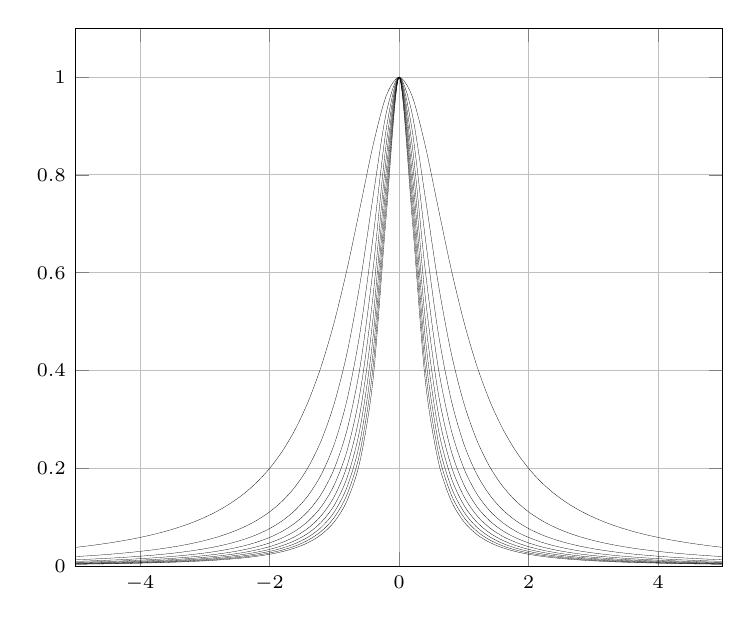
\begin{tikzpicture}
            \begin{axis}[domain=-5:5, restrict y to domain=0:1,
                xmin=-5, xmax=5, ymin=0, ymax=1.1, grid=both,
                tick label style={font=\scriptsize}, xscale=1.2, yscale=1.2]
                \addplot[samples=51,smooth,ultra thin] {1/(1 + 2*x^2)};
                \addplot[samples=51,smooth,ultra thin] {1/(1 + 3*x^2)};
                \addplot[samples=51,smooth,ultra thin] {1/(1 + 4*x^2)};
                \addplot[samples=51,smooth,ultra thin] {1/(1 + 1*x^2)};
                \addplot[samples=51,smooth,ultra thin] {1/(1 + 5*x^2)};
                \addplot[samples=51,smooth,ultra thin] {1/(1 + 6*x^2)};
                \addplot[samples=51,smooth,ultra thin] {1/(1 + 7*x^2)};
                \addplot[samples=51,smooth,ultra thin] {1/(1 + 8*x^2)};
                \addplot[samples=51,smooth,ultra thin] {1/(1 + 9*x^2)};
                \addplot[samples=51,smooth,ultra thin] {1/(1 + 10*x^2)};
            \end{axis}
        \end{tikzpicture}
    \end{figure}
\end{solution}

\subsection{Metryka Czebyszewa}
Weźmy pewną dwuargumentową funkcję zdefiniowaną jako
\[ d_c(f, g) = \sup_{x\in X}\left|f(x) - g(x)\right|. \]
Można udowodnić, że funkcja $d_c$ jest metryką (zwaną metryką Czebyszewa). Jako argumenty przyjmuje dwie funkcja zdefiniowane na tej samej dziedzinie $X$.

\begin{theorem}
    \label{t:uniform convergence iff metric = 0}
    Jeśli każda funkcja ciągu funkcyjnego $(f_n(x))$ jest ograniczona, to
    \[ f_n \rightrightarrows f \Longleftrightarrow \lim_{n\to\infty}d_c(f_n, f) = 0 .\]
\end{theorem}

\begin{example}
    Zbadaj zbieżność punktową i jednostajną ciągu funkcyjnego
    \[ f_n(x) = \frac{x^n}{1 + x^n} \]
    na przedziale $[2, \infty)$.
\end{example}
\begin{solution}
    Mamy
    \[ \lim_{n\to\infty} \frac{x^n}{1 + x^n} = 1 \equiv f, \]
    więc ciąg jest zbieżny punktowo do funkcji ciągłej, możemy zatem sprawdzić, czy zbiega do niej jednostajnie.
    \[ \lim_{n\to\infty}\sup_{x\in X} \left|\frac{x^n}{1 + x^n} - 1\right| = \lim_{n\to\infty}\sup_{x\in X} \left(1 - \frac{x^n}{1 + x^n}\right)\]
    Obliczmy supremum danej funkcji.
    \[ \ddx \left(1 - \frac{x^n}{1 + x^n}\right) = \frac{nx^{n-1}(1 + x^n) - x^n(nx^{n-1})}{\left(1 + x^n\right)^2} = \frac{nx^{n-1}}{\left(1 + x^n\right)^2} \]
    Pochodna zawsze jest dodatnia, więc supremum będzie przy $x \to \infty$. Mamy
    \[ \lim_{n\to\infty}\sup_{x\in X} \left(1 - \frac{x^n}{1 + x^n}\right) = \lim_{n\to\infty}\lim_{x\to\infty} \left(1 - \frac{x^n}{1 + x^n}\right) = \lim_{n\to\infty} \left(1 - 1\right) = 0, \]
    więc dany ciąg jest zbieżny jednostajnie.
\end{solution}

\begin{example}
    Zbadaj zbieżność punktową i jednostajną ciągu funkcyjnego
    \[ f_n(x) = \frac{nx}{n^2 + x^2} \]
    na zbiorze $\RR$.
\end{example}
\begin{solution}
    Mamy
    \[ \lim_{n\to\infty} \frac{nx}{n^2 + x^2} = \lim_{n\to\infty} \frac{x}{n} = 0 \equiv f, \]
    więc ciąg jest zbieżny punktowo do funkcji ciągłej, możemy zatem sprawdzić, czy zbiega do niej jednostajnie.
    \[ \lim_{n\to\infty}\sup_{x\in X} \left|\frac{nx}{n^2 + x^2}\right| = \lim_{n\to\infty}\sup_{x\in X} \left(\frac{nx}{n^2 + x^2}\right) \]
    Obliczmy supremum danej funkcji.
    \[ \ddx \left(\frac{nx}{n^2 + x^2}\right) = \frac{n(n^2 + x^2) - nx(2x)}{\left(n^2 + x^2\right)^2} = \frac{n^3 - nx^2}{\left(n^2 + x^2\right)^2} \]
    Pochodna zeruje się, gdy
    \[ n^3 = nx^2 \implies x = \pm n, \]
    więc supremum będzie przy $x = n$. Mamy
    \[ \lim_{n\to\infty}\frac{n^2}{n^2 + n^2} = \frac{1}{2}, \]
    więc dany ciąg nie jest zbieżny jednostajnie.
\end{solution}

\begin{theorem}[o różniczkowalności granicy ciągu funkcyjnego]
    \label{t:differentiable limit}
    Jeśli każda funkcja ciągu funkcyjnego $(f_n(x))$ jest różniczkowalna, ciąg $(f_n)$ jest zbieżny, a ciąg $(f_n')$ zbieżny jednostajnie, to dla każdego $x \in X$ zachodzi
    \[ \left(\lim_{n\to\infty} f_n(x)\right)' = \lim_{n\to\infty} \left(f_n'(x)\right). \]
\end{theorem}

\begin{theorem}[o całkowalności granicy ciągu funkcyjnego]
    \label{t:integrable limit}
    Jeśli każda funkcja ciągu funkcyjnego $(f_n(x))$ jest całkowalna, a ciąg $(f_n)$ jest zbieżny jednostajnie, to dla każdych $x_1, x_2 \in X$ zachodzi
    \[ \int_{x_1}^{x_2}\left(\lim_{n\to\infty} f_n(x)\right) \d x = \lim_{n\to\infty} \left(\int_{x_1}^{x_2} f_n(x) \d x\right). \]
\end{theorem}

    \section{Szeregi funkcyjne}
    Podobnie do szeregów liczbowych, szeregi funkcyjne to para $((f_n(x))_{n\in\NN}, (S_n(x))_{n\in\NN})$: ciąg funkcyjny oraz ciąg sum częściowych ciągu funkcyjnego. Taki szereg jest zbieżny (punktowo / jednostajnie) do sumy szeregu $S$, jeśli ciąg $(S_n(x))$ jest zbieżny (punktowo / jednostajnie) do $S$.

Analogicznie do twierdzenia \ref{t:uniform convergence implies pointwise convergence}, warunkiem koniecznym zbieżności jednostajnej szeregu jest jego zbieżność punktowa.

Z kolei w analogii do twierdzenia \ref{t:necessary condition of convergence}, warunkiem koniecznym zbieżności (punktowej / jednostajnej) szeregu $\sum_{n=1}^\infty f_n(x)$ jest zbieżność (punktowa / jednostajna) ciągu funkcyjnego $(f_n(x))$ do zera, to znaczy
\[ \sum_{n=1}^\infty f_n(x) \rightarrow S \Longrightarrow f_n(x) \rightarrow 0 \equiv f \]
oraz
\[ \sum_{n=1}^\infty f_n(x) \rightrightarrows S \Longrightarrow f_n(x) \rightrightarrows 0 \equiv f. \]

\begin{theorem}[kryterium Weierstrassa]
    Jeśli istnieje taki ciąg $(a_n)$, że dla każdego $n \in \NN$ i dla każdego $x \in X \subset \RR$ mamy nierówność
    \[ |f_n(x)| \leq a_n \]
    oraz szereg $\sum_{n=1}^\infty a_n$ jest zbieżny, to szereg funkcyjny
    \[ \sum_{n=1}^\infty f_n(x) \]
    jest jednostajnie zbieżny na $X$.
\end{theorem}

Zachodzi twierdzenie o ciągłości, analogiczne do twierdzenia \ref{t:continuous limit}.

\begin{theorem}
    \label{t:continuous series}
    Jeśli szereg $\sum_{n=1}^\infty f_n(x)$ jest szeregiem funkcji ciągłych i jest jednostajnie zbieżny $\sum_{n=1}^\infty f_n(x) \rightrightarrows S(x)$, to funkcja $S$ jest ciągła.
\end{theorem}

\begin{example}
    Zbadaj zbieżność punktową i jednostajną szeregu
    \[ \sum_{n=1}^\infty x^n(1-x) \]
    na przedziale $[0,1]$.
\end{example}
\begin{solution}
    Dla $x \in [0, 1)$ mamy:
    \[ \sum_{n=1}^\infty x^n(1-x) = x(1-x)\frac{1}{1-x} = x, \]
    natomiast dla $x = 1$ mamy
    \[ \sum_{n=1}^\infty x^n(1-x) = \sum_{n=1}^\infty 1^n \cdot 0 = 0, \]
    więc szereg jest zbieżny punktowo. Funkcja
    \[ S(x) = \begin{cases}x, & \text{dla } x \in [0, 1) \\ 0, & \text{dla } x = 1 \end{cases}, \]
    do której dany szereg zbiega, nie jest ciągła, a funkcje $f_n(x) = x^n(1-x)$ są ciągłe, więc, na mocy twierdzenia \ref{t:continuous series}, szereg nie zbiega jednostajnie.
\end{solution}

\begin{example}
    Zbadaj zbieżność punktową i jednostajną szeregu
    \[ \sum_{n=1}^\infty \frac{nx}{1+n^4x^2} \]
    na przedziale $[1,\infty)$.
\end{example}
\begin{solution}
    Dla każdego $x \in [1, \infty]$ oraz $n \in \NN$ mamy
    \[ \left|\frac{nx}{1+n^4x^2}\right| = \frac{nx}{1+n^4x^2} \leq \frac{nx}{n^4x^2} = \frac{1}{n^3x} \leq \frac{1}{n^3}, \]
    więc, na mocy kryterium Weierstrassa, dany szereg jest jednostajnie zbieżny, bo szereg harmoniczny rzędu $3$ jest zbieżny.
\end{solution}

\begin{example}
    Zbadaj obszar zbieżności\footnote{czyli zbiór punktów, w których szereg jest zbieżny} punktowej oraz zbieżność jednostajną szeregu
    \[ \sum_{n=1}^\infty \frac{x^2}{e^{nx}}. \]
\end{example}
\begin{solution}
    Możemy od razu stwierdzić, że dla $x = 0$ otrzymamy szereg ciąg zer, który oczywiście jest (jednostajnie) zbieżny do zera. Możemy potraktować $x$ jako parametr, wtedy, zamiast szeregu funkcyjnego, będziemy mieć szereg liczbowy, którego zbieżność możemy pokazać z kryterium d'Alemberta:
    \[ g = \lim_{n\to\infty} \frac{x^2}{e^{x(n+1)}}\frac{e^{xn}}{x^2} = \lim_{n\to\infty}\frac{1}{e^x} = \frac{1}{e^x}. \]
    Szereg jest więc zbieżny dla każdego $x > 0$ i rozbieżny dla każdego $x < 0$. Ostatecznie, obszar zbieżności punktowej danego szeregu funkcyjnego to $[0,\infty)$.

    Zajmijmy się teraz zbieżnością jednostajną. Oczywiście można by ją wykazywać przez znalezienie ciągu sum częściowych, a następnie skorzystanie z twierdzenia \ref{t:uniform convergence iff metric = 0}, ale możemy też skorzystać z kryterium Weierstrassa, chociaż w dosyć nieoczywisty sposób.

    Znajdźmy najpierw supremum ciągu $a_n = \frac{x^2}{e^{nx}}$. Możemy znaleźć miejsca zerowe pochodnej:
    \[ \ddx \frac{x^2}{e^{nx}} = \frac{2x(e^{nx}) - x^2(ne^{nx})}{e^{2nx}} = \frac{x(2 - xn)}{e^{nx}} = 0 \iff x \in \left\{0, \frac{2}{n}\right\}. \]
    Szkicując wykres pochodnej, przekonamy się, że funkcja $a_n(x)$ osiąga maksimum w $x = \frac{2}{n}$, więc
    \[ a_n(x) \leq a_n\left(\tfrac{2}{n}\right) = \frac{\left(\frac{2}{n}\right)^2}{e^2} = \frac{4}{e^2n^2}. \]
    Szereg $\sum_{n=1}^\infty \frac{4}{e^2n^2}$ jest zbieżny (ponieważ jest harmoniczny rzędu $2$), więc możemy użyć kryterium Weierstrassa udowadniając, że dany szereg funkcyjny jest jednostajnie zbieżny.
\end{solution}

Zachodzą również twierdzenia o różniczkowalności i całkowalności, analogiczne do twierdzeń \ref{t:differentiable limit} i \ref{t:integrable limit}.

\begin{theorem}
    \label{t:differentiable series}
    Niech $(f_n(x))$ będzie ciągiem funkcji różniczkowalnych. Jeśli szereg $\sum_{n=1}^\infty f_n(x)$ jest zbieżny na $X$, a szereg $\sum_{n=1}^\infty f_n'(x)$ jest jednostajnie zbieżny na $X$, to dla każdego $x \in X$ zachodzi
    \[ \left(\sum_{n=1}^\infty f_n(x)\right)' = \sum_{n=1}^\infty f_n'(x). \]
\end{theorem}

\begin{theorem}
    \label{t:integrable series}
    Niech $(f_n(x))$ będzie ciągiem funkcji całkowalnych. Jeśli szereg $\sum_{n=1}^\infty f_n(x)$ jest jednostajnie zbieżny na $X$, to dla każdych $x_1, x_2 \in X$ zachodzi
    \[ \int_{x_1}^{x_2}\left(\sum_{n=1}^\infty f_n(x)\right)\d x = \sum_{n=1}^\infty \left(\int_{x_1}^{x_2}f_n(x)\d x\right). \]
\end{theorem}

\subsection{Szeregi potęgowe}
\begin{definition}
    \label{d:power series}
    Szereg potęgowy o środku w punkcie $c$ to szereg funkcyjny
    \[ \sum_{n=1}^\infty a_n(x - c)^n, \]
    gdzie $a_n, x, c \in \CC$.
\end{definition}

\begin{theorem}
    Jeśli szereg potęgowy
    \[ \sum_{n=1}^\infty a_n(x - c)^n \]
    jest zbieżny dla pewnego $x_1$, to jest zbieżny dla wszystkich $x_2$ takich, że
    \[ |x_2 - c| < |x_1 - c|, \]
    a jeśli nie jest zbieżny dla pewnego $x_1$, to nie jest zbieżny dla wszystkich $x_2$ takich, że
    \[ |x_2 - c| > |x_1 - c|. \]
\end{theorem}

Powyższe twierdzenie każe nam podzielić płaszczyznę zespoloną (względem danego szeregu potęgowego) na trzy rozłączne zbiory. Formalnie, jeśli weźmiemy
\[ r = \sup\left\{|x - c| : \text{ szereg } \sum_{n=1}^\infty a_n(x - c)^n \text{ jest zbieżny}\right\}, \]
to zbiór
\[ \{x \in \CC : |x - x_0| < r\} \]
nazwiemy \vocab{kołem zbieżności}. Dla wszystkich elementów z tego zbioru dany szereg jest zbieżny. Dla elementów na brzegu tego koła zbieżność jest nieokreślona, a dla elementów poza nim dany szereg nie jest zbieżny. Liczba $r$ to \vocab{promień zbieżności}. Dla $x=c$ dany szereg jest zbieżny.

\begin{remark*}
    Jeśli przyjmiemy w definicji szeregu potęgowego (\ref{d:power series}), że $a_n, x, c \in \RR$, to koło zbieżności staje się \vocab{przedziałem zbieżności}, a nieokreśloną zbieżność mamy tylko dla dwóch elementów: $c - r$ oraz $c + r$.
\end{remark*}

\vocab{Obszarem zbieżności} nazywamy zbiór będący sumą koła zbieżności oraz zbioru elementów z jego brzegu, dla których dany szereg potęgowy jest zbieżny.

\begin{theorem}[Cauchy'ego-Hadamarda]
    \label{t:Cauchy-Hadamard}
    Promień zbieżności jest dany jako
    \[ r = \frac{1}{\limsup\limits_{n\to\infty}\sqrt[n]{|a_n|}}, \]
    gdzie $r = \frac{1}{0}$ interpretujemy jako $r = \infty$, a $r = \frac{1}{\infty}$ jako $r = 0$.
\end{theorem}

Można podać dwa słabsze twierdzenia, które jednak często łatwiej jest stosować:
\[ r = \frac{1}{\lim\limits_{n\to\infty} \left|\frac{a_{n+1}}{a_n}\right|} \hspace{1em}\Longrightarrow\hspace{1em} r = \frac{1}{\lim\limits_{n\to\infty}\sqrt[n]{|a_n|}} \hspace{1em}\Longrightarrow\hspace{1em} (\ref{t:Cauchy-Hadamard}). \]

Mówimy, że ciąg (szereg) funkcyjny jest \vocab{niemal jednostajnie zbieżny} na przedziale $(a, b)$, jeśli jest jednostajnie zbieżny na każdym przedziale $[c, d] \in (a, b)$.

\begin{fact}
    Jeśli szereg potęgowy jest zbieżny w $(c-r, c+r)$, to jest bezwzględnie zbieżny w $(c-r, c+r)$ oraz niemal jednostajnie zbieżny w $(c-r, c+r)$.
\end{fact}

\begin{fact}
    Jeśli szereg potęgowy jest zbieżny w $(c-r, c+r)$ do $S(x)$, to funkcja $S(x)$ jest ciągła, różniczkowalna i całkowalna w $(c-r, c+r)$. Prawdziwe dla szeregów potęgowych są również tezy twierdzeń \ref{t:differentiable series} i \ref{t:integrable series}.
\end{fact}

\begin{theorem}[Abela]
    \label{t:Abel}
    Niech $\sum_{n=1}^\infty a_n(x - c)^n$ będzie szeregiem potęgowym zbieżnym do $S(x)$ o promieniu zbieżności równym $r$. Jeśli ten szereg jest zbieżny dla $x_1 = c - r$ oraz istnieje granica $\lim\limits_{x\to x_1^+}S(x)$, to
    \[ \lim_{x\to x_1^+}S(x) = S(x_1), \]
    czyli funkcja $S(x)$ jest prawostronnie ciągła w $x = c - r$. Analogicznie, jeśli szereg jest zbieżny dla $x_2 = c + r$ oraz istnieje granica $\lim\limits_{x\to x_2^-}S(x)$, to
    \[ \lim_{x\to x_2^-}S(x) = S(x_2), \]
    czyli funkcja $S(x)$ jest lewostronnie ciągła w $x = c + r$.
\end{theorem}

\begin{example}
    Znajdź sumę szeregu
    \[ \sum_{n=1}^\infty\frac{(n+1)(x+2)^n}{2^n} \]
    w każdym punkcie obszaru zbieżności.
\end{example}
\begin{solution}
    Stosując twierdzenie Cauchy'ego-Hadamarda (\ref{t:Cauchy-Hadamard}) możemy obliczyć promień zbieżności danego szeregu
    \[ r = \frac{1}{\lim\limits_{n\to\infty}\sqrt[n]{\frac{n+1}{2^n}}} = \frac{1}{\frac{1}{2}} = 2, \]
    tak więc przedział zbieżności to $(-4, 0)$.
    Dla $x = -4$ mamy
    \[ \sum_{n=1}^\infty\frac{(n+1)(-2)^n}{2^n} = \sum_{n=1}^\infty(-1)^n(n+1) \text{ -- rozbieżny, nie spełnia warunku koniecznego}, \]
    a dla $x = 0$
    \[ \sum_{n=1}^\infty\frac{(n+1)2^n}{2^n} = \sum_{n=1}(n+1) \text{ -- rozbieżny, nie spełnia warunku koniecznego}. \]
    Obszarem zbieżności jest więc przedział $(-4, 0)$. Policzmy teraz sumę. Dla każdego $x \in (-4, 0)$ mamy
    \begin{align*}
        S(x) &= \sum_{n=1}^\infty\frac{(n+1)(x+2)^n}{2^n} = \sum_{n=1}^\infty \left(\frac{(x+2)^{n+1}}{2^n}\right)' \overset{(\ref{t:differentiable series})}{=} \left(\sum_{n=1}^\infty\frac{(x+2)^{n+1}}{2^n}\right)' \\
        &= \left(\frac{(x+2)^2}{2}\frac{1}{1 - \frac{x+2}{2}}\right)' = \left(\frac{(x+2)^2}{-x}\right)' = \frac{-2x(x+2) + (x+2)^2}{x^2} = \frac{4 - x^2}{x^2}.
    \end{align*}
\end{solution}

\begin{example}
    Znajdź sumę szeregu
    \[ \sum_{n=0}^\infty \frac{2^n(x - \frac{1}{2})^n}{n+1} \]
    w każdym punkcie obszaru zbieżności.
\end{example}
\begin{solution}
    Stosując twierdzenie Cauchy'ego-Hadamarda (\ref{t:Cauchy-Hadamard}) możemy obliczyć promień zbieżności danego szeregu
    \[ r = \frac{1}{\lim\limits_{n\to\infty}\sqrt[n]{\frac{2^n}{n+1}}} = \frac{1}{2}, \]
    tak więc przedział zbieżności to $(0, 1)$.
    Dla $x = 0$ mamy
    \[ \sum_{n=0}^\infty \frac{2^n\left(-\frac{1}{2}\right)^n}{n+1} = \sum_{n=0}^\infty \frac{(-1)^n}{n+1} \text{ -- zbieżny z kryterium Leibniza}, \]
    a dla $x = 1$
    \[ \sum_{n=0}^\infty \frac{2^n\left(\frac{1}{2}\right)^n}{n+1} = \sum_{n=0}^\infty \frac{1}{n+1} \text{ -- rozbieżny z kryterium ilorazowego}. \]
    Obszarem zbieżności jest więc przedział $[0, 1)$. Policzmy teraz sumę. Dla $x = \frac{1}{2}$ mamy
    \[ S(\tfrac{1}{2}) = \sum_{n=0}^\infty \frac{2^n0^n}{n+1} = 1 + 0 + 0 + \cdots = 1. \]
    Dla pozostałych $x$ zapiszemy
    \[ S(x) = \sum_{n=0}^\infty \frac{2^n(x - \frac{1}{2})^n}{n+1} = \frac{1}{x - \frac{1}{2}}\sum_{n=0}^\infty \frac{2^n(x - \frac{1}{2})^{n+1}}{n+1} = \frac{1}{x - \frac{1}{2}}\sum_{n=0}^\infty \int_{\frac{1}{2}}^x 2^n\left(t-\frac{1}{2}\right)^n\d t. \]
    Szeregi potęgowe są niemal jednostajnie zbieżne w swoim przedziale zbieżności, więc dla $x \in (0, 1)$ możemy zamienić znaki sumy i całki (twierdzenie \ref{t:integrable series})
    \begin{align*}
        S(x) &= \frac{1}{x - \frac{1}{2}}\int_{\frac{1}{2}}^x \sum_{n=0}^\infty 2^n\left(t-\frac{1}{2}\right)^n\d t = \frac{1}{x - \frac{1}{2}}\int_{\frac{1}{2}}^x \frac{1}{1 - 2(t - \frac{1}{2})}\d t \\
        &= \frac{1}{x - \frac{1}{2}}\int_{\frac{1}{2}}^x \frac{1}{2 - 2t}\d t = \frac{1}{x - \frac{1}{2}}\left[-\frac{1}{2}\ln(1 - t)\right]_{\frac{1}{2}}^x = \frac{1}{1 - 2x}\left(\ln(1 - x) - \ln{\frac{1}{2}}\right) \\
        &= \frac{\ln(2 - 2x)}{1 - 2x}.
    \end{align*}
    Z twierdzenia Abela (\ref{t:Abel}) wynika, że
    \[ S(0) = \lim_{x\to 0^+}\frac{\ln(2 - 2x)}{1 - 2x} = \ln(2), \]
    więc ostatecznie mamy
    \[ S(x) = \begin{cases}1, & \text{dla } x = \tfrac{1}{2} \\ \frac{\ln(2 - 2x)}{1 - 2x}, & \text{dla } x \in [0, 1)\setminus \{\tfrac{1}{2}\} \end{cases}. \]
\end{solution}

\begin{example}
    Znajdź sumę szeregu liczbowego
    \[ 1 - \frac{1}{3} + \frac{1}{5} - \frac{1}{7} + \ldots. \]
\end{example}
\begin{solution}
    Weźmy szereg funkcyjny
    \[ S(x) = \sum_{n=0}^\infty \frac{(-1)^n}{2n+1}x^{2n+1}. \]
    Wartość $S(1)$ jest szukaną sumą, jeśli tylko szereg jest zbieżny w tym punkcie. Niech $t = x^2$. Stosując twierdzenie Cauchy'ego-Hadamarda (\ref{t:Cauchy-Hadamard}) możemy obliczyć promień zbieżności szeregu:
    \[ r_t = \frac{1}{\lim\limits_{n\to\infty}\frac{2n+1}{2n+3}} = 1, \]
    tak więc szereg zbiega, gdy $t \in (-1, 1) \implies x \in (-1, 1)$. W punktach $x = -1$ i $x = 1$ szereg również jest zbieżny, co można pokazać z kryterium Leibniza.

    Policzmy teraz sumę (dla przedziału zbieżności $(-1, 1)$):
    \begin{align*}
        S(x) &= \sum_{n=0}^\infty \frac{(-1)^n}{2n+1}x^{2n+1} = \sum_{n=0}^\infty\int_0^x (-1)^n u^{2n} \d u = \int_0^x\sum_{n=0}^\infty (-1)^n u^{2n} \d u \\
        &= \int_0^x\sum_{n=0}^\infty (-u^2)^n \d u = \int_0^x \frac{1}{1 + u^2} \d u = \Big[\arctan(u)\Big]_0^x = \arctan(x).
    \end{align*}

    Skoro w $x = 1$ ten szereg też jest zbieżny, to z twierdzenia Abela (\ref{t:Abel}) mamy
    \[ S(1) = \lim_{x\to 1}\arctan(x) = \arctan(1) = \frac{\pi}{4}. \]
\end{solution}
        \subsection{Szeregi Taylora}
        \begin{theorem}[o rozwijaniu funkcji w szereg Taylora]
    Jeśli funkcja $f$ ma pochodne wszystkich rzędów w pewnym otoczeniu $U$ punktu $x_0$, to na pewnym przedziale zachodzi równość
    \[ f(x) = \sum_{n=0}^\infty \frac{f^{(n)}(x_0)}{n!}(x - x_0)^n. \]
    Taki szereg nazywamy szeregiem Taylora, a jeśli $x_0 = 0$, to nazywamy go szeregiem Maclaurina.
\end{theorem}

\begin{fact}
    Dosyć łatwo wyprowadzić następujące rozwinięcia w szeregi Maclaurina, które mogą być użyteczne w zadaniach:
    \[ \frac{1}{1 - x} = \sum_{n=0}^\infty x^n, x \in (-1, 1) \]
    \[ e^x = \sum_{n=0}^\infty \frac{x^n}{n!}, x \in \RR \]
    \[ \sin{x} = \sum_{n=0}^\infty \frac{(-1)^n x^{2n+1}}{(2n+1)!}, x \in \RR \]
    \[ \cos{x} = \sum_{n=0}^\infty \frac{(-1)^n x^{2n}}{(2n)!}, x \in \RR \]
\end{fact}

\begin{example}
    Rozwiń w szereg Taylora funkcję $f(x) = \ln{x}$ w otoczeniu $x_0 = 1$.
\end{example}
\begin{solution}
    Spróbujmy znaleźć ogólny wzór na $f^{(n)}(x)$. Mamy
    \begin{align*}
        f'(x) &= \frac{1}{x} \\
        f''(x) &= \frac{-1}{x^2} \\
        f'''(x) &= \frac{2}{x^2} \\
        f^{(4)}(x) &= \frac{-6}{x^3} \\
        &\ldots \\
        f^{(n)}(x) &= (-1)^{n+1}\frac{(n-1)!}{x^n} \\
        &\implies f^{(n)}(1) = (-1)^{n+1}(n-1)!,
    \end{align*}
    tak więc
    \[ f(x) = \sum_{n=0}^\infty \frac{(-1)^{n+1}(n-1)!}{n!}(x-1)^n = \frac{(-1)^{n+1}}{n}(x-1)^n. \]
    Z twierdzenia Cauchy'ego-Hadamarda (\ref{t:Cauchy-Hadamard})
    \[ r = \frac{1}{\lim\limits_{n\to\infty}\frac{n}{n+1}} = 1 \]
    wynika, że ten szereg jest zbieżny, a więc równość jest prawdziwa, dla każdego $x \in (0, 2)$. Łatwo sprawdzić (z kryterium Leibniza), że jest zbieżny też dla $x = 2$, więc (z twierdzenia Abela) również dla $x = 2$ równość jest prawdziwa.
\end{solution}

\begin{example}
    Rozwiń w szereg Maclaurina funkcję $f(x) = x^3\arctan{x^4}$.
\end{example}
\begin{solution}
    Weźmy $g(x) = \arctan{x^4}$. Mamy
    \[ g'(x) = \frac{4x^3}{1 + x^8} = \frac{4x^3}{1 - (-x^8)}, \hspace{2em} |x^8| < 1 \implies x \in (-1, 1) \]
    więc
    \[ g'(x) = \sum_{n=0}^\infty 4x^3 (-x^8)^n = \sum_{n=0}^\infty (-1)^n 4x^{8n+3}, \]
    ergo
    \begin{align*}
        g(x) &= \int_0^x g'(t) \d t = \int_0^x\sum_{n=0}^\infty (-1)^n 4t^{8n+3} \d t \\
        &= \sum_{n=0}^\infty (-1)^n 4 \int_0^x t^{8n+3} \d t = \sum_{n=0}^\infty (-1)^n \frac{4x^{8n+4}}{8n+4}.
    \end{align*}
    Ostatecznie mamy
    \[ f(x) = \sum_{n=0}^\infty \frac{(-1)^n}{2n+1}x^{8n+7}. \]
    Równość jest prawdziwa dla $x \in (-1, 1)$ oraz (z kryterium Leibniza i twierdzenia Abela) dla $x = \pm 1$.
\end{solution}
        \subsection{Szeregi Fouriera}
        Zbiór funkcji \vocab{całkowalnych z kwadratem} będziemy oznaczać przez $L^2[a, b]$. Formalnie
\[ L^2[a, b] = \left\{f: [a, b] \to \RR : \int\limits_{[a, b]} f^2(x) \d x < \infty \right\}. \]
Jeśli utożsamimy ze sobą funkcje, które różnią się zbiorze miary Riemanna równej zero, to struktura $(L^2[a, b], \RR, +, \cdot)$ jest przestrzenią wektorową, w której możemy wprowadzić iloczyn skalarny
\[ f \circ g = \int\limits_{[a, b]} f(x)g(x) \d x. \]
Mamy więc przestrzeń unitarną, ergo zdefiniowana jest w niej też norma
\[ \Vert f \Vert = \sqrt{f \circ f} = \sqrt{\int_a^b f^2(x) \d x} \]
oraz metryka
\[ d(f, g) = \Vert f - g \Vert = \sqrt{\int_a^b \left(f(x) - g(x)\right)^2 \d x}. \]
Zbieżność w sensie metryki $d$ to \vocab{zbieżność przeciętna z kwadratem}.

\begin{definition}
    Ciąg ortogonalny to taki ciąg funkcyjny $(\varphi_n)_{n\geq 0}$, którego funkcje nie są tożsamościowo równe zeru, są całkowalne z kwadratem oraz jego elementy są prostopadłe, czyli
    \[ \dforall{i \neq j} \varphi_i \circ \varphi_j = 0. \]
\end{definition}

\begin{definition}
    Ciąg ortonormalny to taki ciąg ortogonalny, że jego elementy są wersorami, czyli
    \[ \dforall{i, j} \varphi_i \circ \varphi_j = \begin{cases}1, & \text{dla } i = j \\ 0, & \text{dla } i \neq j\end{cases}. \]
    Wartość $\varphi_i \circ \varphi_j$ oznaczamy $\delta_{ij}$ i nazywamy \vocab{deltą Kroneckera}.
\end{definition}

\vocab{Szeregiem ortogonalnym} będziemy nazywać szereg funkcyjny w postaci $\sum_{n=0}^\infty c_n\varphi_n$, gdzie $(c_n)$ jest ciągiem liczb rzeczywistych, a $(\varphi_n)$ ciągiem ortogonalnym.

\begin{theorem}[współczynniki Eulera-Fouriera]
    \label{t:Euler-Fourier}
    Jeśli szereg
    \[ \sum_{n=0}^\infty c_n\varphi_n \rightrightarrows f \]
    jest ortogonalny i zbiega jednostajnie do funkcji $f \in L^2[a, b]$, to dla każdego $n \in \NN$
    \[ c_n = \frac{f \circ \varphi_n}{\Vert \varphi_n \Vert^2}. \]
\end{theorem}

\begin{proof}
    Niech
    \[ f(x) = \sum_{n=0}^\infty c_n\varphi_n. \]
    Wybierzmy dowolne $m \in \NN$. Mamy
    \begin{align*}
        f(x) \cdot \varphi_m (x)
        &= \sum_{n=0}^\infty c_n \varphi_n(x) \cdot \varphi_m(x), \\
        \int_a^b f(x) \varphi_m(x) \d x
        &= \int_a^b \sum_{n=0}^\infty c_n \varphi_n(x) \varphi_m(x) \d x.
    \end{align*}
    Skoro szereg jest zbieżny jednostajnie, to (korzystając z twierdzenia \ref{t:integrable series}) możemy zamienić znaki sumy i całki, otrzymując
    \[ \int_a^b f(x) \varphi_m(x) \d x = \sum_{n=0}^\infty c_n \int_a^b \varphi_n(x) \varphi_m(x) \d x, \]
    a ponieważ $(\varphi_n)_{n \in \NN}$ jest ciągiem ortogonalnym (czyli dla $n \neq m$, $\int_a^b \varphi_n(x) \varphi_m(x) = 0$), suma sprowadza się do
    \begin{align*}
        \int_a^b f(x) \varphi_m(x) \d x
        &= c_m \int_a^b \varphi_m(x) \varphi_m(x) \d x \\
        f \circ \varphi_m
        &= c_m \cdot (\varphi_m \circ \varphi_m)
        = c_m \cdot \Vert \varphi_m \Vert^2 \\
        \frac{f \circ \varphi_m}{\Vert \varphi_m \Vert^2}
        &= c_m.
    \end{align*}
\end{proof}

Szereg ortogonalny, w którym współczynniki mają powyższą formę, nazywamy \vocab{szeregiem Fouriera} funkcji $f$. Oznaczamy
\[ f \sim \sum_{n=0}^\infty c_n\varphi_n. \]
Jeśli powyższy szereg ortogonalny jest zbieżny do $f$ na całym przedziale $[a, b]$, to mówimy, że ta funkcja jest \vocab{rozwijalna} w szereg Fouriera.

\begin{theorem}[nierówność Bessela]
    Jeśli szereg
    \[ \sum_{n=0}^\infty c_n\varphi_n \]
    jest szeregiem Fouriera funkcji $f$ względem ciągu $(\varphi_n)$, to
    \[ \Vert f \Vert^2 \geq \sum_{n=0}^\infty c_n^2 \Vert \varphi_n \Vert^2. \]
\end{theorem}

\begin{theorem}[tożsamość Parsevala]
    \label{t:Parseval}
    Jeśli szereg
    \[ \sum_{n=0}^\infty c_n\varphi_n \]
    jest szeregiem Fouriera funkcji $f$ względem ciągu $(\varphi_n)$, to
    \[ \Vert f \Vert^2 = \sum_{n=0}^\infty c_n^2 \Vert \varphi_n \Vert^2 \]
    wtedy i tylko wtedy, gdy $\sum_{n=0}^\infty c_n\varphi_n$ jest przeciętnie zbieżny z kwadratem do $f$.
\end{theorem}

Jeśli pewien szereg spełnia tożsamość Parsevala dla każdej funkcji $f \in L^2[a, b]$, to mówimy, że ciąg $(\varphi_n)$ jest \vocab{zupełny}.

\begin{corollary}
    Jeśli ciąg $(\varphi_n)$ jest zupełny oraz $f \sim \sum_{n=0}^\infty c_n\varphi_n$, to szereg
    \[ \sum_{n=0}^\infty c_n\varphi_n \]
    jest przeciętnie zbieżny z kwadratem do $f$ na $[a, b]$.
\end{corollary}

\subsection{Trygonometryczne szeregi Fouriera}
\begin{fact}
    Ciąg
    \[ 1, \cos x, \sin x, \cos 2x, \sin 2x, \ldots, \cos nx, \sin nx, \ldots \]
    jest zupełny (a więc i ortogonalny).
\end{fact}

\begin{corollary}[współczynniki Eulera-Fouriera (\ref{t:Euler-Fourier}) dla szeregów trygonometrycznych]
    \label{c:Euler-Fourier for trig}
    Szeregiem trygonometrycznym Fouriera funkcji całkowalnej $f : [-\pi, \pi] \to \RR$ będziemy nazywać szereg
    \[ \frac{a_0}{2} + \sum_{n=1}^\infty a_n\cos nx + b_n\sin nx, \]
    gdzie
    \begin{align*}
        a_0 &= \frac{1}{\pi}\int_{-\pi}^\pi f(x) \d x \\
        a_n &= \frac{1}{\pi}\int_{-\pi}^\pi f(x)\cos nx \d x \\
        b_n &= \frac{1}{\pi}\int_{-\pi}^\pi f(x)\sin nx \d x.
    \end{align*}
\end{corollary}

\begin{definition}[warunki Dirichleta] ~
    \begin{enumerate}
        \item funkcja $f : [a, b] \to \RR$ jest ograniczona,
        \item funkcja $f$ ma skończoną liczbę przedziałów monotoniczności,
        \item funkcja $f$ ma skończoną liczbę punktów nieciągłości $x_0$ oraz
        \[ f(x_0) = \frac{\lim\limits_{x\to x_0^-}f(x) + \lim\limits_{x\to x_0^+}f(x)}{2}, \]
        \item zachodzi równość
        \[ f(a) = f(b) = \frac{\lim\limits_{x\to a^+}f(x) + \lim\limits_{x\to b^-}f(x)}{2}. \]
    \end{enumerate}
\end{definition}

\begin{theorem}[o rozwijaniu funkcji w szereg Fouriera]
    Jeśli funkcja $f$ spełnia warunki Dirichleta w przedziale $[-\pi, \pi]$, to szereg trygonometryczny Fouriera tej funkcji jest zbieżny punktowo do $f$ na $[-\pi, \pi]$.
\end{theorem}

\begin{remark}
    Jeśli funkcja $f$ spełnia warunki Dirichleta w przedziale $[-\pi, \pi]$ oraz jest nieparzysta, to
    \[ f(x) = \sum_{n=1}^\infty b_n\sin nx, \]
    gdzie $b_n = \frac{2}{\pi}\int_0^\pi f(x)\sin nx \d x$. Jeśli jest parzysta, to
    \[ f(x) = \frac{a_0}{2} + \sum_{n=1}^\infty a_n\cos nx, \]
    gdzie $a_n = \frac{2}{\pi}\int_0^\pi f(x)\cos nx \d x$. Tworzą one wtedy odpowiednio szereg sinusów i cosinusów.
\end{remark}

\begin{example}
    Rozwiń w szereg Fouriera funkcję
    \[ f(x) = \begin{cases}
        0, & \text{dla } x \in (-\pi, 0) \\
        x, & \text{dla } x \in [0, \pi)
    \end{cases}. \]
    Korzystając z niego, oblicz sumę szeregu liczbowego $1 + \frac{1}{3^2} + \frac{1}{5^2} + \ldots$.
\end{example}
\begin{solution}
    Aby funkcja $f$ spełniała wszystkie warunki Dirichleta, musimy dodać wartość w punkcie $x = \pm \pi$.
    \[ f(-\pi) = f(\pi) = \frac{\lim\limits_{x\to -\pi^+}f(x) + \lim\limits_{x\to \pi^-}f(x)}{2} = \frac{0 + \pi}{2} = \frac{\pi}{2}. \]
    Możemy więc już napisać
    \[ f(x) = \frac{a_0}{2} + \sum_{n=1}^\infty a_n\cos nx + b_n\sin nx, \]
    gdzie
    \begin{align*}
        a_0 &= \frac{1}{\pi}\int_{-\pi}^\pi f(x) \d x = \frac{1}{\pi}\left(\int_{-\pi}^0 0 \d x + \int_0^\pi x \d x\right) = \frac{1}{\pi}\left(\frac{\pi^2}{2}\right) = \frac{\pi}{2}, \\
        a_n &= \frac{1}{\pi}\int_{-\pi}^\pi f(x)\cos{nx} \d x = \frac{1}{\pi}\left(\int_{-\pi}^0 0 \d x + \int_0^\pi x \cos{nx} \d x\right) = \\
            &= \frac{1}{\pi}\left(\left[\frac{nx\sin{nx} + \cos{nx}}{n^2}\right]_0^\pi\right) = \frac{n\pi\sin{n\pi} + \cos{n\pi}}{\pi n^2} = \frac{\cos{n\pi} - 1}{\pi n^2} = \frac{(-1)^n - 1}{\pi n^2}, \\
        b_n &= \frac{1}{\pi}\int_{-\pi}^\pi f(x)\sin{nx} \d x = \frac{1}{\pi}\left(\int_{-\pi}^0 0 \d x + \int_0^\pi x \sin{nx} \d x\right) = \\
            &= \frac{1}{\pi}\left(\left[\frac{-nx\cos{nx} + \sin{nx}}{n^2}\right]_0^\pi\right) = \frac{1}{\pi}\frac{\sin{n\pi} - n\pi\cos{n\pi}}{n} = \frac{-\cos{n\pi}}{n} = \frac{(-1)^{n+1}}{n}.
    \end{align*}
    Mamy więc
    \[ f(x) = \frac{\pi}{4} + \sum_{n=1}^\infty \frac{(-1)^n - 1}{\pi n^2}\cos{nx} + \frac{(-1)^{n+1}}{n}\sin{nx}. \]
    W punkcie $x = \pi$:
    \[ f(\pi) = \frac{\pi}{4} + \sum_{n=1}^\infty \frac{(-1)^n - 1}{\pi n^2}(-1)^n = \frac{\pi}{4} + \sum_{n=1}^\infty \frac{1 - (-1)^n}{\pi n^2} = \frac{\pi}{4} + \frac{2}{\pi}\left(1 + \frac{1}{3^2} + \frac{1}{5^2} + \ldots\right), \]
    ergo
    \[ 1 + \frac{1}{3^2} + \frac{1}{5^2} + \ldots = \frac{\pi}{2}\left(f(\pi) - \frac{\pi}{4}\right) = \frac{\pi}{2}\left(\frac{\pi}{2} - \frac{\pi}{4}\right) = \frac{\pi^2}{8}. \]
\end{solution}

\begin{corollary}[tożsamość Parsevala (\ref{t:Parseval}) dla szeregów trygonometrycznych]
    Przyjmujemy oznaczenia jak we wniosku \ref{c:Euler-Fourier for trig}. Zachodzi równość
    \[ \frac{1}{\pi}\int_{-\pi}^\pi \left(f(x)\right)^2 \d x = \frac{a_0^2}{2} + \sum_{n=1}^\infty a_n^2 + b_n^2. \]
\end{corollary}

\begin{example}
    Rozwiń w szereg Fouriera funkcję
    \[ f(x) = x^2 \]
    dla $x \in [-\pi, \pi]$. Korzystając z tego rozwinięcia, oblicz sumę szeregów liczbowych
    \[ \sum_{n=1}^\infty \frac{1}{n^2} \text{ oraz } \sum_{n=1}^\infty \frac{1}{n^4}. \]
\end{example}
\begin{solution}
    \href{https://www.youtube.com/watch?v=2VYBGF_MPIU}{blackpenredpen na YouTube}. Wynik to odpowiednio $\frac{\pi^2}{6}$ i $\frac{\pi^4}{90}$.
\end{solution}


    \section{Rachunek różniczkowy funkcji wielu zmiennych}
    W tej sekcji będziemy skupiać się na funkcjach typu $\RR^k \to \RR$. W tym kontekście warto zauważyć, że struktura $(\RR^k, \RR, +, \cdot)$ jest przestrzenią wektorową. Jest ona również przestrzenią Banacha ze zdefiniowaną normą euklidesową.

\begin{fact}[granica ciągu]
    Weźmy ciąg $(x_n)$ elementów zbioru $\RR^k$ i oznaczmy $x_n = (x_{n,1}, x_{n,2}, \ldots, x_{n,k})$. Zachodzi równoważność
    \[ \lim_{n\to\infty} x_n = (g_1, g_2, \ldots, g_k) \iff \dforall{1\leq i\leq k} \lim_{n\to\infty}x_{n,i} = g_i. \]
\end{fact}

\begin{definition}[Heinego]
    Funkcja $f : D \to \RR$, gdzie $D\subset\RR^k$, ma granicę w punkcie $x_0$ równą $g$ wtedy i tylko wtedy, gdy dla każdego ciągu $(x_n)$ takiego, że $x_n \in D, x_n \neq x_0$ oraz $\lim_{n\to\infty} x_n = x_0$ zachodzi
    \[ \lim_{n\to\infty} f(x_n) = g. \]
\end{definition}

\begin{example}
    Zbadaj granicę
    \[ \lim_{(x, y)\to (0, 0)} \frac{x^2}{x^2 + y^2}. \]
\end{example}
\begin{solution}
    Podstawiając $x = 0$ mamy
    \[ \lim_{y\to 0} \frac{0}{0 + y^2} = 0, \]
    a dla $y = 0$ otrzymujemy
    \[ \lim_{x\to 0} \frac{x^2}{x^2 + 0} = 1, \]
    więc granica nie istnieje. Bardziej formalnie możemy powiedzieć, że wzięliśmy dwa ciągi: $a_n = (0, \frac{1}{n}), b_n = (\frac{1}{n}, 0)$ i pokazaliśmy sprzeczność z definicją Heinego.
\end{solution}

\begin{figure}[H]
    \centering
    \begin{tikzpicture}[scale=0.8]
        \begin{axis}[my axis style, view = {20}{30}]
            \addplot3[
                domain = -2:2, domain y = -2:2,
                samples = 30, samples y = 30,
                surf, opacity=.4
            ]{x^2/(x^2 + y^2)};
        \end{axis}
    \end{tikzpicture}
    \caption{Wykres funkcji $f(x, y) = \frac{x^2}{x^2 + y^2}$.}
\end{figure}

\begin{example}
    Zbadaj granicę
    \[ \lim_{(x, y)\to (0, 0)} \frac{\sin(x^2 + y^2)}{x^2 + y^2}. \]
\end{example}
\begin{solution}
    \begin{align*}
        &\lim_{(x, y)\to (0, 0)} \frac{\sin(x^2 + y^2)}{x^2 + y^2} = \left|\begin{alignedat}{2}&x = r\cos\varphi \\ &y = r\sin\varphi\end{alignedat}\right| = \lim_{r\to 0} \frac{\sin(r^2\cos^2\varphi + r^2\sin^2\varphi)}{r^2\cos^2\varphi + r^2\sin^2\varphi} = \\
        &= \lim_{r\to 0} \frac{\sin(r^2)}{r^2} = \lim_{t\to 0} \frac{\sin t}{t} = 1.
    \end{align*}
\end{solution}

\begin{figure}[H]
    \centering
    \begin{tikzpicture}[scale=0.8]
        \begin{axis}[my axis style, view = {20}{30}]
            \addplot3[
                domain = -2:2, domain y = -2:2,
                samples = 30, samples y = 30,
                surf, opacity=.4
            ]{sin(deg(x^2 + y^2))/(x^2 + y^2)};
        \end{axis}
    \end{tikzpicture}
    \caption{Wykres funkcji $f(x, y) = \frac{\sin(x^2 + y^2)}{x^2 + y^2}$.}
\end{figure}

\begin{example}
    Zbadaj granicę
    \[ \lim_{(x, y)\to (0, 0)} \frac{xy^2}{x^2 + y^2}. \]
\end{example}
\begin{solution}
    Skoro
    \[ 0 \leq \left|\frac{xy^2}{x^2 + y^2}\right| = |x|\frac{y^2}{x^2 + y^2} \leq |x| \]
    oraz $\lim_{(x, y)\to (0, 0)} 0 = \lim_{(x, y)\to (0, 0)} |x| = 0$, to, na mocy twierdzenia o trzech ciągach,
    \[ \lim_{(x, y)\to (0, 0)} \left|\frac{xy^2}{x^2 + y^2}\right| = 0, \]
    więc
    \[ \lim_{(x, y)\to (0, 0)} \frac{xy^2}{x^2 + y^2} = 0. \]
\end{solution}

\begin{figure}[H]
    \centering
    \begin{tikzpicture}[scale=0.8]
        \begin{axis}[my axis style, view = {-15}{30}]
            \addplot3[
                domain = -2:2, domain y = -2:2,
                samples = 30, samples y = 30,
                surf, opacity=.4
            ]{(x * y^2)/(x^2 + y^2)};
        \end{axis}
    \end{tikzpicture}
    \caption{Wykres funkcji $f(x, y) = \frac{xy^2}{x^2 + y^2}$.}
\end{figure}

\begin{example}
    Zbadaj granicę
    \[ \lim_{(x, y)\to (0, 0)} \frac{xy^2}{x^2 + y^4} \]
\end{example}
\begin{solution}
    Podstawiając $y = x$ mamy
    \[ \lim_{x\to 0} \frac{x^3}{x^2 + x^4} = 0, \]
    a dla $x = y^2$ otrzymujemy
    \[ \lim_{y\to 0} \frac{y^4}{y^4 + y^4} = \frac{1}{2}, \]
    więc granica nie istnieje.
\end{solution}

\begin{remark*}
    Powyższy przykład jest o tyle ciekawy, że jeśli $x$ oraz $y$ zbiegają w tym samym tempie (czyli łączy jest liniowa zależność) to zawsze granica wyjdzie zerowa. Aby pokazać ten fakt, przejdziemy do współrzędnych biegunowych:
    \[ \lim_{(x, y)\to (0, 0)} \frac{xy^2}{x^2 + y^4}  = \lim_{r\to 0} \frac{r^3 \cos\varphi\sin^2\varphi}{r^2\cos^2\varphi + r^4\sin^4\varphi} = \lim_{r\to 0} \frac{r \cos\varphi\sin^2\varphi}{\cos^2\varphi + r^2\sin^4\varphi}. \]
    Jeśli $\varphi = \pm\frac{\pi}{2}$, to (skoro $\cos\varphi = 0$)
    \[ \lim_{r\to 0} \frac{r \cos\varphi\sin^2\varphi}{\cos^2\varphi + r^2\sin^4\varphi} = \lim_{r\to 0} \frac{0}{0 \pm r^2} = 0, \]
    a jeśli $\varphi \neq \pm\frac{\pi}{2}$, to (skoro $\sin$ i $\cos$ są ograniczone)
    \[ \lim_{r\to 0} \frac{r \cos\varphi\sin^2\varphi}{\cos^2\varphi + r^2\sin^4\varphi} = \frac{0}{\cos^2\varphi + 0} = 0. \]

    Natomiast jeśli $\varphi$ nie jest stałe, ale na przykład zbiega do $\frac{\pi}{2}$, to, jak można zauważyć na poniższym rysunku, granica niekoniecznie będzie zerowa.
\end{remark*}

\begin{figure}[H]
    \centering
    \begin{tikzpicture}[scale=0.8]
        \begin{axis}[my axis style, view = {-10}{40}]
            \addplot3[
                thick, AccColor4, samples=10,
                domain=-1:1,
            ]({x},{x/3},{x*(x/3)^2/(x^2 + (x/3)^4)});
            \addplot3[
                domain = -1:1, domain y = -1:1,
                samples = 30, samples y = 30,
                surf, opacity=.4
            ]{x*y^2/(x^2 + y^4)};
        \end{axis}
    \end{tikzpicture}
    \begin{tikzpicture}[scale=0.8]
        \begin{axis}[my axis style, view = {0}{0}]
            \addplot3[
                domain = -1:1, domain y = -1:1,
                samples = 30, samples y = 30,
                surf, opacity=.4
            ]{x*y^2/(x^2 + y^4)};
            \addplot3[
                thick, AccColor4, samples=10,
                domain=-1:1,
            ]({x},{x/3},{x*(x/3)^2/(x^2 + (x/3)^4)});
        \end{axis}
    \end{tikzpicture}
    \caption[short]{Wykres funkcji $f(x, y) = \frac{xy^2}{x^2 + y^4}$ z zaznaczoną prostą $y = \frac{x}{3}$.}
\end{figure}

Granicę funkcji $f(x, y)$ w formie $\lim_{(x, y) \to (x_0, y_0)} f(x, y)$ nazywamy czasami \vocab{granicą podwójną}\footnote{co może być nazwą mylącą; w literaturze angielskiej jest to \textit{ordinary limit}, który nie jest tym samym pojęciem co \textit{double limit}. W szczególności dla \textit{double limit} nie zachodzi fakt \ref{f:iterated and ordinary limit}, zobacz też: \href{https://en.wikipedia.org/wiki/Iterated_limit\#Limit_of_function}{wikipedia}.}, w odróżnieniu od granic $\lim_{x\to x_0} \lim_{y\to y_0} f(x, y)$ czy $\lim_{y\to y_0} \lim_{x\to x_0} f(x, y)$, które są \vocab{granicami iterowanymi}.

\begin{fact}
    \label{f:iterated and ordinary limit}
    Jeśli funkcja $f(x, y)$ ma w punkcie $(x_0, y_0)$ granicę podwójną oraz istnieją obie jej granice iterowane, to wszystkie trzy są sobie równe.
\end{fact}
\begin{proof}[Uzasadnienie]
    Granica iterowana w punkcie $(x_0, y_0)$ modeluje dążenie do tego punktu po dwóch bokach prostokąta.
\end{proof}

\begin{remark*}
    Jeśli obie granice iterowane nie istnieją, to nie znaczy, że granica podwójna nie istnieje. Jeśli obie granice iterowanie istnieją i są sobie równe, to nie znaczy, że granica podwójna istnieje.

    Natomiast z powyższego faktu wynika, że jeśli obie granice iterowane istnieją i nie są sobie równe, to granica podwójna nie istnieje.
\end{remark*}

\begin{fact}
    Jeśli funkcja (wielu zmiennych) $f$ jest ciągła w $x_0$, a funkcja $g$ jest ciągła w~$f(x_0)$, to funkcja $g\circ f$ jest ciągła w $x_0$.
\end{fact}

\begin{fact}
    Jeśli funkcje (wielu zmiennych) $f, g$ są ciągłe w $x_0$, to funkcje $f+g, f-g, f\cdot g$ również są ciągłe w tym punkcie. Jeśli dodamy warunek, że $g(x) \neq 0$ dla pewnego otoczenia $x_0$, to ciągła w tym puncie jest również funkcja $\frac{f}{g}$.
\end{fact}
        \subsection{Pochodne funkcji wielu zmiennych}
        \begin{definition}
    Pochodną funkcji $f : \RR^k \supset D \to \RR^m$ wzdłuż wektora $\vec{v}$ nazwiemy taką funkcję $D_v f$, że
    \[ D_v f(x) = \lim_{t\to 0}\frac{f(x + t\vec{v}) - f(x)}{t}. \]
\end{definition}

Oprócz notacji Eulera ($D_v f$) stosuje się również notację Leibniza ($D_v f(x) = \frac{\p f(x)}{\p{\vec{v}}})$ oraz  Lagrange'a ($f'_{\vec{v}}$).

Pochodna \vocab{w kierunku} wektora $\vec{v}$ jest pochodną wzdłuż wektora $\frac{\vec{v}}{\Vert\vec{v}\Vert}$. Te pojęcia są oczywiście równoważne, jeśli $\vec{v}$ jest wersorem. Najczęściej używamy jednak \vocab{pochodnych cząstkowych}, to znaczy pochodnych wzdłuż wersorów osiowych, oznaczając
\[ \frac{\p f}{\p x}(x, y) = \frac{\p f}{\p [1, 0]}(x, y) \hspace{1em}\text{ oraz }\hspace{1em} \frac{\p f}{\p y}(x, y) = \frac{\p f}{\p [0, 1]}(x, y). \]

\begin{definition}[różniczka]
    Funkcja $f : \RR^k \supset D \to \RR^m$ jest różniczkowalna w $p$, gdy istnieje takie przekształcenie liniowe $L_{p} : \RR^k \to \RR^m$, że dla każdego $p + h$ w otoczeniu $p$ zachodzi
    \[ \lim_{h\to\vec{0}} \frac{f(p + h) - f(p) - L_{p}(h)}{\Vert h \Vert} = \vec{0}. \]
    Funkcję $L_{p}(h)$ nazywamy różniczką funkcji $f$ w punkcie $p$ i oznaczamy $\d f(p)(h)$.
\end{definition}

\begin{theorem}[warunek konieczny różniczkowalności]
    \label{t:differentiability implies derivability}
    Jeśli funkcja $f : \RR^k \supset D \to \RR^m$ jest różniczkowalna w punkcie $p$, to istnieje pochodna funkcji $f$ w punkcie $p$ wzdłuż dowolnego wektora $h \in \RR^k$ i zachodzi
    \[ \frac{\p f}{\p h}(p) = \d f(p)(h). \]
\end{theorem}
\begin{proof}[Wyprowadzenie wzoru]
    Pamiętając, że $\d f(p)$ jest przekształceniem liniowym, więc może być rozpatrywane jako macierz, możemy równoważnie stwierdzić, że
    \[ \lim_{h\to\vec{0}} \frac{f(p + h) - f(p) - \d f(p) \cdot h}{\Vert h \Vert} = \vec{0} \]
    \[ \lim_{t\to 0} \frac{f(p + th) - f(p) - \d f(p) \cdot th}{t} = \vec{0} \]
    \[ \lim_{t\to 0} \frac{f(p + th) - f(p)}{t} = \d f(p)\cdot h \]
    \[ \frac{\p f}{\p h}(p) = \d f(p)\cdot h. \]
\end{proof}

\begin{definition}[jakobian]
    Dana jest funkcja $f : \RR^k \supset D \to \RR^m$, gdzie
    \[ f(p) = f(x_1, \ldots, x_k) = (f_1(x_1, \ldots, x_k), \ldots, f_m(x_1, \ldots, x_k)).\]
    Macierz
    \[ \d f(p) = \begin{bNiceMatrix}
        \frac{\p f_1}{\p x_1}(p) & \frac{\p f_1}{\p x_2}(p) & \Cdots & \frac{\p f_1}{\p x_k}(p) \\
        \frac{\p f_2}{\p x_1}(p) & \frac{\p f_2}{\p x_2}(p) & \Cdots & \frac{\p f_2}{\p x_k}(p) \\
        \Vdots & \Vdots & \Ddots & \Vdots \\
        \frac{\p f_m}{\p x_1}(p) & \frac{\p f_m}{\p x_2}(p) & \Cdots & \frac{\p f_m}{\p x_k}(p) \\
    \end{bNiceMatrix} \]
     nazywamy \vocab{macierzą Jacobiego} funkcji $f$ w punkcie $p$. Jeśli macierz ta jest kwadratowa, to jej wyznacznik nazywamy jakobianem funkcji $f$ w punkcie $p$ i oznaczamy $J(p)$.
\end{definition}

Chcąc obliczyć różniczkę $\d f(p)$ w punkcie $h$ wystarczy pomnożyć macierz $\d f(p)$ i~wektor $h$, więc
\[ \d f(p)(h) = \begin{bNiceMatrix}
    \frac{\p f_1}{\p x_1}(p) & \frac{\p f_1}{\p x_2}(p) & \Cdots & \frac{\p f_1}{\p x_k}(p) \\
    \frac{\p f_2}{\p x_1}(p) & \frac{\p f_2}{\p x_2}(p) & \Cdots & \frac{\p f_2}{\p x_k}(p) \\
    \Vdots & \Vdots & \Ddots & \Vdots \\
    \frac{\p f_m}{\p x_1}(p) & \frac{\p f_m}{\p x_2}(p) & \Cdots & \frac{\p f_m}{\p x_k}(p) \\
\end{bNiceMatrix}\begin{bNiceMatrix}
    h_1 \\ h_2 \\ \Vdots \\ h_k
\end{bNiceMatrix} = \begin{bNiceMatrix}
    \frac{\p f_1}{\p x}(p)h_1 \\ \frac{\p f_2}{\p x}(p)h_2 \\ \Vdots \\ \frac{\p f_m}{\p x}(p)h_k
\end{bNiceMatrix} \]

\begin{theorem}[warunek konieczny różniczkowalności]
    Jeśli funkcja jest różniczkowalna w $x_0$, to jest ciągła w $x_0$.
\end{theorem}

\begin{theorem}[warunek wystarczający różniczkowalności]
    \label{t:differentiability of multivar functions}
    Jeśli istnieją i są ciągłe wszystkie pochodne cząstkowe funkcji $f$ w punkcie $x_0$, to funkcja $f$ jest różniczkowalna w $x_0$.
\end{theorem}

\begin{example}
    Zbadaj różniczkowalność funkcji
    \[ f(x, y) = \begin{cases}\frac{x^3 + y^3}{x^2 + x^2}, & \text{dla } (x, y) \neq (0, 0) \\ 0, & \text{w przeciwnym wypadku}\end{cases} \]
    w całej jej dziedzinie.
\end{example}
\begin{solution}
    Skorzystajmy z warunku wystarczającego na różniczkowalność funkcji. Pochodne cząstkowe
    \[ \frac{\p{}}{\p x}\left(\frac{x^3 + y^3}{x^2 + x^2}\right) = \frac{(3x^2)(x^2 + y^2) - (x^3 + y^3)(2x)}{(x^2 + y^2)^2} \]
    \[ \frac{\p{}}{\p y}\left(\frac{x^3 + y^3}{x^2 + x^2}\right) = \frac{(3y^2)(x^2 + y^2) - (x^3 + y^3)(2y)}{(x^2 + y^2)^2} \]
    są ciągłe w $\RR^2 \setminus \{(0, 0)\}$, więc w tym zbiorze funkcja $f$ jest różniczkowalna. Aby sprawdzić, czy funkcja jest również różniczkowalna w $p = (0, 0)$ policzymy pochodną w tym punkcie w kierunku wersora $h$:
    \begin{align*}
        &\lim_{t\to 0}\frac{f(p+th) - f(p)}{t} = \lim_{t\to 0}\frac{f(th)}{t} = \lim_{t\to 0}\frac{\frac{t^3\cos^3\varphi + t^3\sin^3\varphi}{t^2\cos^2\varphi + t^2\sin^2\varphi}}{t} = \\
        =& \lim_{t\to 0}\frac{t^3\cos^3\varphi + t^3\sin^3\varphi}{t^3} = \cos^3\varphi + \sin^3\varphi = h_1^3 + h_2^3.
    \end{align*}
    Na mocy warunku koniecznego różniczkowalności (\ref{t:differentiability implies derivability}) funkcja $f$ nie jest różniczkowalna w $(0, 0)$, ponieważ pochodna w kierunku $h$ powinna być wynikiem przekształcenia \textbf{liniowego} wektora $h$.
\end{solution}
\begin{solution}
    Pierwsza część alternatywnego rozwiązania przebiega tak samo, więc zbadamy tylko różniczkowalność funkcji $f$ w punkcie $(0, 0)$. Z definicji różniczki i macierzy Jacobiego mamy
    \[ \lim_{h\to\vec{0}} \frac{f(p + h) - f(p) - L_{p}(h)}{\Vert h \Vert} = \lim_{h\to\vec{0}} \frac{f(h) - L_{p}(h)}{\Vert h \Vert} = \lim_{h\to\vec{0}} \frac{\frac{h_1^3 + h_2^3}{h_1^2 + h_2^2} - \frac{\p f(0, 0)}{\p x}h_1 - \frac{\p f(0, 0)}{\p y}h_2}{\Vert h \Vert}. \]
    Możemy policzyć z definicji pochodnej
    \[ \frac{\p f(0, 0)}{\p x} = \lim_{t\to 0}\frac{f(t, 0) - f(0, 0)}{t} = \frac{\frac{t^3}{t^2}}{t} = 1 \]
    \[ \frac{\p f(0, 0)}{\p y} = \lim_{t\to 0}\frac{f(0, t) - f(0, 0)}{t} = \frac{\frac{t^3}{t^2}}{t} = 1, \]
    więc
    \begin{align*}
        &\lim_{h\to\vec{0}} \frac{\frac{h_1^3 + h_2^3}{h_1^2 + h_2^2} - \frac{\p f(0, 0)}{\p x}h_1 - \frac{\p f(0, 0)}{\p y}h_2}{\Vert h \Vert} = \lim_{h\to\vec{0}} \frac{\frac{h_1^3 + h_2^3}{h_1^2 + h_2^2} - h_1 - h_2}{\Vert h \Vert} = \\
        =& \lim_{r\to 0}\frac{\frac{r^3(\cos^3\varphi + \sin^3\varphi)}{r^2} - r\cos\varphi - r\sin\varphi}{r} = \cos^3\varphi + \sin^3\varphi - \cos\varphi + \sin\varphi \neq 0,
    \end{align*}
    więc funkcja $f$ nie jest różniczkowalna w $(0, 0)$.
\end{solution}

\begin{remark}
    Warunek wystarczający (\ref{t:differentiability of multivar functions}) nie jest równocześnie warunkiem koniecznym (to znaczy, że twierdzenie nie jest tożsamością). Przykładem niech będzie funkcja
    \[ f(x, y) = \begin{cases}(x^2 + y^2)\sin\left(\frac{1}{\sqrt{x^2 + x^2}}\right), & \text{dla } (x, y) \neq (0, 0) \\ 0, & \text{w przeciwnym wypadku}\end{cases}. \]
\end{remark}

W przypadku funkcji $\RR \to \RR$ różniczkowalność w punkcie znaczy, że istnieje styczna do wykresu funkcji w tym punkcie. W podobny sposób możemy zinterpretować geometrycznie różniczkowalność funkcji $\RR^2 \to \RR$: funkcja jest różniczkowalna w punkcie, gdy w tym punkcie istnieje płaszczyzna styczna do wykresu funkcji. Taka płaszczyzna będzie mieć równanie
\begin{equation}
    z = f(x_0, y_0) + \frac{\p f}{\p x}(x_0, y_0) \cdot (x - x_0) + \frac{\p f}{\p y}(x_0, y_0) \cdot (y -y_0).
\end{equation}

\begin{example}
    Znajdź równanie płaszczyzny stycznej do funkcji
    \[ f(x, y) = e^{x^2 - y} \]
    w punkcie $p = (1, 0)$.
\end{example}
\begin{solution}
    Najpierw znajdźmy pochodne cząstkowe:
    \begin{align*}
        \frac{\p f}{\p x}f(x, y) = e^{x^2 - y} \cdot 2x = 2xe^{x^2 - y} \\
        \frac{\p f}{\p y}f(x, y) = e^{x^2 - y} \cdot (-1) = -e^{x^2 - y}.
    \end{align*}
    Płaszczyzna styczna w punkcie $p$ ma więc wzór
    \[ z  = e^{1 - 0} + 2\cdot 1\cdot e^{1 - 0}\cdot (x - 1) - e^{1 - 0}\cdot (y - 0) \]
    \[ z  = 2ex - ey - e. \]
\end{solution}

\begin{figure}[H]
    \centering
    \begin{tikzpicture}[scale=0.8]
        \begin{axis}[my axis style, view = {-15}{30}]
            \addplot3[colormap={CM}{color=(AccColor3) color=(AccColor3)},
                domain = -1.5:1.5, domain y = -1.5:1.5,
                samples = 10, samples y = 10,
                surf, opacity=0.3
            ]{e*(2*x - y - 1)};
            \addplot3[
                domain = -1.5:1.5, domain y = -1.5:1.5,
                samples = 30, samples y = 30,
                surf, opacity=.4
            ]{exp(x^2 - y)};
            \node[draw=none, shape=circle, fill, opacity=0.8, AccColor1, inner sep=1.5pt] (d1) at (1,0,e){};
        \end{axis}
    \end{tikzpicture}
    \begin{tikzpicture}[scale=0.8]
        \begin{axis}[my axis style, view = {10}{10}]
            \addplot3[colormap={CM}{color=(AccColor3) color=(AccColor3)},
                domain = -1.5:1.5, domain y = -1.5:1.5,
                samples = 10, samples y = 10,
                surf, opacity=0.3, 
            ]{e*(2*x - y - 1)};
            \addplot3[
                domain = -1.5:1.5, domain y = -1.5:1.5,
                samples = 30, samples y = 30,
                surf, opacity=.4
            ]{exp(x^2 - y)};
            \node[draw=none, shape=circle, fill, opacity=0.8, AccColor1, inner sep=1.5pt] (d1) at (1,0,e){};
        \end{axis}
    \end{tikzpicture}
    \caption{Wykres funkcji $f(x, y) = e^{x^2 - y}$ z płaszczyzną styczną w $(1, 0)$.}
\end{figure}

Również analogicznie do funkcji $\RR \to \RR$ możemy za pomocą pochodnych przybliżać wartości funkcji $\RR^k \to \RR$. Mamy
\begin{equation}
    f(x_0 + h) \approx f(x_0) + \d f(x_0)(h),
\end{equation}
jeśli tylko funkcja $f$ jest różniczkowalna w otoczeniu $x_0$.

Pochodna cząstkowa \vocab{drugiego rzędu} to pochodna
\[ \frac{\p{}^2 f}{\p x_j \p x_i} = \frac{\p{}}{\p x_j}\left(\frac{\p f}{\p x_i}\right). \]
Jeśli $i = j$, czyli pochodna ma postać $\frac{\p{}^2 f}{\p{} x^2}$, to nazywamy ją pochodną \vocab{czystą}, a przeciwnym wypadku jest \vocab{mieszana}.

Analogicznie do twierdzenia \ref{t:differentiability of multivar functions} funkcja $f: D \supset \RR^k \to \RR^m$ jest \vocab{$2$-krotnie różniczkowalna} w punkcie $p$, gdy istnieją i są ciągłe wszystkie (jest ich $k^2$) pochodne cząstkowe $2$-go rzędu funkcji $f$ w punkcie $p$.

\begin{theorem}[Schwarza o pochodnych mieszanych]
    Jeśli funkcja $f$ jest $2$-krotnie różniczkowalna w $p$, to
    \[ \frac{\p{}^2 f}{\p x \p y}(p) = \frac{\p{}^2 f}{\p y \p x}(p). \]
\end{theorem}

Jeśli funkcja $f:\RR^2 \to \RR$ jest $2$-krotnie różniczkowalna, to możemy zdefiniować różniczkę $2$-go rzędu:
\begin{align*}
    &\d{}^2 f(h_1, h_2) = \d{} \left(\frac{\p f}{\p x} h_1 + \frac{\p f}{\p y} h_2\right) = \frac{\p f}{\p x}\left(\frac{\p f}{\p x} h_1 + \frac{\p f}{\p y} h_2\right)h_1 + \frac{\p f}{\p y}\left(\frac{\p f}{\p x} h_1 + \frac{\p f}{\p y} h_2\right)h_2 \\
    &= \frac{\p{}^2 f}{\p x^2} + 2\frac{\p f}{\p x\p y} + \frac{\p{}^2 f}{\p y^2}.
\end{align*}
        \subsection{Ekstrema lokalne}
        \begin{definition}[maksimum lokalne]
    \label{d:local maximum}
    Funkcja $f : D \to \RR$ określona na obszarze $D \subset \RR^n$ ma maksimum lokalne w punkcie $x_0 \in D$, jeśli istnieje takie sąsiedztwo $U \subset D$ punktu $x_0$, że dla każdego $x \in U$
    \[ f(x) < f(x_0). \]
\end{definition}

Analogicznie definiujemy minimum lokalne.

\begin{theorem}[warunek konieczny istnienia ekstremum lokalnego]
    \label{t:necessity for local extrema of differentiable function}
    Jeśli funkcja $f$ jest różniczkowalna oraz ma ekstremum lokalne w $x_0$, to
    \[ \d f(x_0) = \mathbf{0}. \]
\end{theorem}


\begin{definition}
    Forma kwadratowa to funkcja $\varphi : \RR^n \to \RR$ taka, że
    \begin{align*}
        \varphi(x_1, x_2, \ldots, x_n) = a_{11}x_1^2 + a_{12}x_1x_2 + \ldots + a_{1n}x_1x_n \\
            + a_{21}x_{2}x_2 + a_{22}x_2^2 + \ldots + a_{2n}x_2x_n \\
            + \ldots + \ldots + a_nnx_n^2
    \end{align*}
    \[ \varphi(x_1, x_2, \ldots, x_n) = \begin{bNiceMatrix}
        x_1 & \Cdots & x_n
    \end{bNiceMatrix}\begin{bNiceMatrix}
        a_{11} & \Cdots & a_{1n} \\
        \Vdots & \Ddots & \Vdots \\
        a_{n1} & \Cdots & a_{nn}
    \end{bNiceMatrix}\begin{bNiceMatrix}
        x_1 \\ \Vdots \\ x_n
    \end{bNiceMatrix} = X^T \cdot A \cdot X, \]
    gdzie macierz $A$ jest symetryczną macierzą, którą nazywamy \vocab{macierzą formy kwadratowej}. Forma kwadratowa $\varphi$ jest \vocab{określona} dodatnio / ujemnie / nieujemnie / niedodatnio, jeśli dla każdego niezerowego $h \in \RR^n$, $\varphi(h)$ jest dodatnie / ujemne / nieujemne / niedodatnie. Jeśli istnieją dwa wektory, dla których $\varphi$ przyjmuje niezerowe wartości różnych znaków, to mówimy, że forma jest nieokreślona.
\end{definition}

\begin{theorem}[Sylvestera]
    Jeśli $A$ jest macierzą formy kwadratowej $\varphi$ oraz
    \[ d_k = \det \begin{bNiceMatrix}
        a_{11} & \Cdots & a_{1k} \\
        \Vdots & \Ddots & \Vdots \\
        a_{k1} & \Cdots & a_{kk}
    \end{bNiceMatrix}, \]
    jest ciągiem minorów wiodących, to:
    \begin{enumerate}
        \item $\forall_k\ d_k > 0 \implies \varphi$ jest dodatnio określona
        \item $\forall_k\ (-1)^k d_k > 0 \implies \varphi$ jest ujemnie określona
        \item $\forall_k\ d_k \geq 0 \implies \varphi$ jest nieujemnie określona
        \item $\forall_k\ (-1)^k d_k \geq 0 \implies \varphi$ jest niedodatnio określona
        \item w innym wypadku $\varphi$ jest nieokreślona
    \end{enumerate}
\end{theorem}

\begin{definition}[hesjan]
    Jeśli funkcja $f : \RR^n \supset D \to \RR$ jest dwukrotnie różniczkowalna w punkcie $p$, to macierz
    \[ H(p) = \begin{bNiceMatrix}
        \frac{\p{}^2 f}{\p x_1^2}(p) & \frac{\p{}^2 f}{\p x_1 \p x_2}(p) & \Cdots & \frac{\p{}^2 f}{\p x_1 \p x_n}(p) \\
        \frac{\p{}^2 f}{\p x_2 \p x_1}(p) & \frac{\p{}^2 f}{\p x_2^2}(p) & \Cdots & \frac{\p{}^2 f}{\p x_2 \p x_n}(p) \\
        \Vdots & \Vdots & \Ddots & \Vdots \\
        \frac{\p{}^2 f}{\p x_n \p x_1}(p) & \frac{\p{}^2 f}{\p x_n \p x_2}(p) & \Cdots & \frac{\p{}^2 f}{\p x_n^2}(p) \\
    \end{bNiceMatrix} \]
    nazywamy \vocab{macierzą Hessego} (lub po prostu \vocab{hesjanem}) funkcji $f$ w punkcie $p$.
\end{definition}

\begin{theorem}[warunek wystarczający istnienia ekstremum lokalnego]
    \label{t:local extrema with Hessian matrix}
    Dana jest funkcja $f : D \to \RR$ określona na obszarze $D \subset \RR^n$. Jeśli wszystkie jej pochodne cząstkowe drugiego rzędu są ciągłe w pewnym otoczeniu $U \ni p$ oraz spełniony jest warunek konieczny (\ref{t:necessity for local extrema of differentiable function}), to jeśli forma kwadratowa, której macierzą jest macierz Hessego funkcji $f$ w punkcie $p$ jest:
    \begin{enumerate}
        \item określona dodatnio, to istnieje minimum lokalne w punkcie $p$,
        \item określona ujemnie, to istnieje maksimum lokalne w punkcie $p$,
        \item nieokreślona, to nie ma ekstremum lokalnego w punkcie $p$.
    \end{enumerate}
\end{theorem}

\begin{remark}
    Punkty dziedziny, w których różniczka jest tożsamościowa równa zeru lub nie istnieje to \vocab{punkty krytyczne}. Te, które spełniają pierwszy warunek, to \vocab{punkty stacjonarne}. Z warunku koniecznego istnienia ekstremum lokalnego (twierdzenie \ref{t:necessity for local extrema of differentiable function}) wynika, że ekstrema istnieją tylko w punktach krytycznych, jednak nie w każdym punkcie krytycznym jest ekstremum. Takie punkty stacjonarne, w których nie ma minimum ani maksimum, to \vocab{punkty siodłowe}.

    Z warunku wystarczającego istnienia ekstremum lokalnego (twierdzenie \ref{t:local extrema with Hessian matrix}) wynika, że jeśli badamy punkty stacjonarne za pomocą macierzy Hessego i wyjdzie nam chociaż jeden minor zerowy, a forma będzie określona nieujemnie lub niedodatnio, to ta metoda okaże się po prostu nieskuteczna. W szczególności, jeśli badamy funkcję dwóch zmiennych i wyznacznik macierzy Hessego wyjdzie zerowy, to nie możemy nic powiedzieć o istnieniu ekstremum.
\end{remark}

\begin{example}
    \label{ex:x^3 + y^3 - 3xy}
    Znajdź ekstrema lokalne funkcji
    \[ f(x, y) = x^3 + y^3 - 3xy. \]
    \graphref{p8w}
\end{example}
\begin{solution}
    Najpierw policzmy pochodne cząstkowe:
    \[ \frac{\p f}{\p x}(x, y) = 3x^2 - 3y, \qquad \frac{\p f}{\p y}(x, y) = 3y^2 - 3x.\]
    Są one ciągłe, więc funkcja jest różniczkowalna (z \ref{t:differentiability of multivar functions}), więc ewentualne ekstrema na pewno będą w miejscach zerowania się obu pochodnych cząstkowych (z \ref{t:necessity for local extrema of differentiable function}). Mamy więc
    \[ \begin{cases} 3x^2 - 3y = 0 \\ 3y^2 - 3x = 0 \end{cases} \implies \begin{cases} x^2 = y \\ y^2 = x \end{cases} \implies (x, y) \in \{(0, 0), (1, 1)\}. \]

    Policzmy macierz Hessego:
    \[ H(x, y) = \begin{bmatrix}
        \frac{\p{}^2 f}{\p x^2}(x, y) & \frac{\p{}^2 f}{\p x \p y}(x, y) \\
        \frac{\p{}^2 f}{\p y \p x}(x, y) & \frac{\p{}^2 f}{\p y^2}(x, y)
    \end{bmatrix} = \begin{bmatrix}
        \frac{\p{} }{\p x}(3x^2 - 3y) & \frac{\p{} }{\p x}(3y^2 - 3x) \\
        \frac{\p{} }{\p y}(3x^2 - 3y) & \frac{\p{} }{\p y}(3y^2 - 3x)
    \end{bmatrix} = \begin{bmatrix}
        6x & -3 \\
        -3 & 6y
    \end{bmatrix}. \]

    Dla punktu $(x, y) = (1, 1)$ mamy
    \[ H(1, 1) = \begin{bmatrix}
        6 & -3 \\
        -3 & 6
    \end{bmatrix} \implies \begin{cases} d_1 = 6 > 0,\\ d_2 = 6\cdot 6 - 3\cdot 3 > 0 \end{cases}, \]
    więc na podstawie warunku wystarczającego (\ref{t:local extrema with Hessian matrix}) wnioskujemy, że w punkcie $(1, 1)$ jest minimum lokalne.

    Dla punktu $(x, y) = (0, 0)$ mamy
    \[ H(0, 0) = \begin{bmatrix}
        0 & -3 \\
        -3 & 0
    \end{bmatrix} \implies \begin{cases} d_1 = 0,\\ d_2 = -9 < 0 \end{cases}, \]
    więc twierdzenie \ref{t:local extrema with Hessian matrix} mówi, że nie ma tutaj ekstremum lokalnego. Możemy ten fakt również sprawdzić w inny sposób -- zauważmy, że
    \[ f(\eps, 0) = \eps^3 \]
    przyjmuje wartości większe od $f(0, 0) = 0$ dla $\eps > 0$ oraz mniejsze dla $\eps < 0$, więc punkt $(0, 0)$ jest punktem siodłowym.
\end{solution}

\begin{figure}[H]
    \centering
    \begin{tikzpicture}[scale=0.8]
        \begin{axis}[my axis style, view = {-20}{30}]
            \addplot3[
                domain = -0.5:1.4, domain y = -0.5:1.4,
                samples = 30, samples y = 30,
                surf, opacity=.4
            ]{x^3 + y^3 - 3*x*y};
        \end{axis}
    \end{tikzpicture}
    \caption{Wykres funkcji $f(x, y) = x^3 + y^3 - 3xy$.}
\end{figure}

\begin{example}
    Znaleźć odległość punktu $A = (0, 1, 0)$ od powierzchni $\pi : y = xz$.
\end{example}
\begin{solution}
    Weźmy punkt $P \in \pi$. Wtedy $P = (x, xz, z)$, a odległość tego punktu od punktu $A$ wyraża się wzorem
    \[ f(x, z) = \sqrt{x^2 + (xz- 1)^2 + z^2}. \]
    Możemy skorzystać z faktu, że funkcja pierwiastkowa jest monotoniczna i spróbować znaleźć minimum funkcji
    \[ g(x, z) = x^2 + (xz - 1)^2 + z^2. \]
    Pochodne cząstkowe
    \[ \frac{\p g(x, z)}{\p x} = 2x + 2xz^2 - 2z, \qquad \frac{\p g(x, z)}{\p z} = 2z + 2x^2z - 2x \]
    są ciągłe, więc funkcja $g$ jest różniczkowalna, więc jej minimum może być jedynie w punktach stacjonarnych:
    \[ \begin{cases} x + xz^2 - z = 0 \\ z + x^2z - x = 0 \end{cases}. \]
    Po dodaniu stronami i podstawieniu odpowiednich wartości przekształcamy powyższy układ równań do
    \[ x = z = 0. \]
    Przyjemność zweryfikowania, że metoda macierzy Hessego dla tego puntu nie rozstrzygnie istnienia minimum pozostawione jest Czytelnikowi.

    W takiej sytuacji musimy poradzić sobie jakoś inaczej. Wykorzystując nierówność między średnimi (AM-GM) mamy:
    \[ g(x, z) = x^2 + z^2 + (xz - 1)^2 \geq 2\sqrt{x^2z^2} + (xz)^2 - 2xz + 1 = (xz)^2 + 1 \geq 1. \]
    Aby zamiast słabych nierówności mogły pojawić się tutaj równości, musi być spełnione $x^2 = z^2$ (z AM-GM) oraz $xz = 0$. To oczywiście zachodzi dla $x = z = 0$, więc pokazaliśmy, że $d_e(A, \pi) = \sqrt{1} = 1$.
\end{solution}

Warto zauważyć, że zamiast sprawdzać, kiedy słabe nierówności są równościami, można było również po prostu policzyć odległość punktu $A$ od punktu $P = (0, 0, 0)$, ponieważ wiemy, że tylko w nim może wystąpić minimum.
        \subsection{Ekstrema warunkowe}
        \begin{definition}[maksimum warunkowe]
    Funkcja $f : \RR^n \supset S \to \RR$ ma maksimum warunkowe w punkcie $x_0 \in D$ przy warunku $g : D \to \RR$, jeśli istnieje takie sąsiedztwo $U \subset D$ punktu $x_0$, że dla każdego $x \in U \cap S$
    \[ f(x) < f(x_0), \]
    przy
    \[ S = \{x \in D : g(x) = 0\}. \]
\end{definition}

Analogicznie definiujemy minimum warunkowe.

\begin{remark*}
    W przeciwieństwie do definicji ekstremum lokalnego (definicja \ref{d:local maximum}) nie wymagamy, żeby zbiór $S$ był otwarty i spójny (był obszarem). Nie możemy więc bezpośrednio stosować twierdzeń i metod z poprzedniej sekcji.
\end{remark*}

\begin{theorem}[Weierstrassa o osiąganiu kresów]
    \label{t:Weierstrass}
    Jeśli funkcja $f : D \to \RR$ jest ciągła, a zbiór $D \in \RR^n$ jest zwarty, to funkcja $f$ osiąga swoje kresy, czyli istnieją takie $x_1, x_2 \in D$, że dla każdego $x \in D$ zachodzi
    \[ f(x_1) \leq f(x) \leq f(x_2). \]
\end{theorem}

Zachodzi twierdzenie analogiczne do twierdzenia \ref{t:necessity for local extrema of differentiable function}:

\begin{theorem}[warunek konieczny istnienia ekstremum warunkowego]
    \label{t:necessity for conditional extrema of differentiable function}
    Jeśli funkcje $f, g$ są różniczkowalne w sposób ciągły oraz $f$ ma ekstremum warunkowe w punkcie $x_0$ przy warunku $g$, to istnieje takie $\lambda \in \RR$, że
    \[ \d L(x_0, \lambda) = \symbf{0}, \]
    gdzie $L(x, \lambda) = f(x) + \lambda g(x)$ to funkcja Lagrange'a.
\end{theorem}

\begin{definition}[hesjan obrzeżony]
    Jeśli funkcja $f : \RR^n \supset D \to \RR$ jest dwukrotnie różniczkowalna w sposób ciągły w punkcie $p$, to macierz
    \[ H(p, \lambda) = \begin{bNiceMatrix}
        0 & \frac{\p g}{\p x_1}(p) & \frac{\p g}{\p x_2}(p) & \Cdots & \frac{\p g}{\p x_n}(p) \\
        \frac{\p g}{\p x_1}(p) & \frac{\p{}^2 L}{\p x_1^2}(p, \lambda) & \frac{\p{}^2 L}{\p x_1 \p x_2}(p, \lambda) & \Cdots & \frac{\p{}^2 L}{\p x_1 \p x_n}(p, \lambda) \\
        \frac{\p g}{\p x_2}(p) & \frac{\p{}^2 L}{\p x_2 \p x_1}(p, \lambda) & \frac{\p{}^2 L}{\p x_2^2}(p, \lambda) & \Cdots & \frac{\p{}^2 L}{\p x_2 \p x_n}(p, \lambda) \\
        \Vdots & \Vdots & \Vdots & \Ddots & \Vdots \\
        \frac{\p g}{\p x_n}(p) & \frac{\p{}^2 L}{\p x_n \p x_1}(p, \lambda) & \frac{\p{}^2 L}{\p x_n \p x_2}(p, \lambda) & \Cdots & \frac{\p{}^2 L}{\p x_n \p x_n}(p, \lambda)
    \end{bNiceMatrix} \]
    nazywamy \vocab{hesjanem obrzeżonym} funkcji $f$ w punkcie $p$.
\end{definition}

Analogicznie do twierdzenia \ref{t:local extrema with Hessian matrix} mamy:

\begin{theorem}[warunek wystarczający istnienia ekstremum warunkowego]
    \label{t:conditional extrema with Hessian matrix}
    Dane są funkcje $f : S \to \RR$ oraz $g : D \to \RR$, gdzie $S \subset D \subset \RR^n$. Jeśli wszystkie ich pochodne cząstkowe drugiego rzędu są ciągłe w pewnym otoczeniu $U \ni p$ oraz spełniony jest warunek konieczny (\ref{t:necessity for conditional extrema of differentiable function}) dla punktu $(p, \lambda)$, to
    \begin{enumerate}
        \item $\forall_{k = 2, \ldots, n}\ d_k < 0 \implies$ istnieje minimum warunkowe w punkcie $p$,
        \item $\forall_{k = 2, \ldots, n}\ (-1)^{k+1} d_k < 0 \implies$ istnieje maksimum warunkowe w punkcie $p$,
        \item jeśli nie zachodzi warunek $\forall_k\ d_k \leq 0$ ani $\forall_k\ (-1)^{k+1} d_k \leq 0$, to nie ma ekstremum lokalnego w punkcie $p$,
    \end{enumerate}
    gdzie $d_k$ jest wyznacznikiem minora wiodącego hesjanu obrzeżonego o rozmiarze $(k+1)$.
\end{theorem}

\begin{example}
    Znajdź maksymalną wartość funkcji
    \[ f(x, y) = x^2 + xy + 2y - x \]
    na zbiorze
    \[ S = \{(x, y) \in \RR^2 : x^2 \leq y \leq 6\}. \]
    \graphref{b4a}
\end{example}

\begin{solution}
    Najpierw policzmy pochodne cząstkowe:
    \[ \frac{\p f(x, y)}{\p x} = 2x + y - 1, \qquad \frac{\p f(x, y)}{\p y} = x + 2. \]

    W zbiorze $S_1 = \{(x, y) \in \RR^2 : x^2 < y < 6\} \subset S$ (który jest obszarem) funkcja przyjmuje ewentualne maksimum lokalne, tylko gdy obie pochodne się zerują (na podstawie twierdzenia \ref{t:necessity for local extrema of differentiable function}), więc
    \[ \begin{cases} 2x + y - 1 = 0 \\ x + 2 = 0 \end{cases} \implies (x, y) = (-2, 5) \in S_1. \]
    Hesjan ma postać
    \[ H(x, y) = \begin{bmatrix}
        2 & 1 \\
        1 & 0
    \end{bmatrix} \implies \begin{cases} d_1 = 2 > 0 \\ d_2 = -1 < 0 \end{cases}, \]
    więc (z twierdzenia \ref{t:local extrema with Hessian matrix}) punkt $(-2, 5)$ jest punktem siodłowym, a na zbiorze $S_1$ funkcja $f$ nie przyjmuje maksimum.

    Sprawdźmy teraz zbiór $S_2 = \{(x, y) \in \RR^2 : x^2 = y < 6\} \subset S$. Możemy posłużyć się funkcją Lagrange'a:
    \[ L(x, y, \lambda) = f(x, y) + \lambda g(x, y), \qquad g(x, y) = x^2 - y. \]
    Z twierdzenie \ref{t:necessity for conditional extrema of differentiable function} maksimum warunkowe może istnieć, tylko gdy
    \[ \frac{\p L(x, y, \lambda)}{\p x} = 2x + y - 1 + \lambda(2x) = 0, \qquad \frac{\p L(x, y, \lambda)}{\p y} = x + 2 - \lambda = 0 \]
    \[ \implies \begin{cases} 2x + y - 1 + 2\lambda x = 0 \\ \lambda = x + 2 \\ y = x^2 \end{cases} \implies \begin{cases} 2x + x^2 - 1 + 2(x+2)x = 0 \\ \lambda = x + 2 \\ y = x^2 \end{cases}. \]
    Pierwsze równanie z układu przyjmuje postać
    \[ 3x^2 + 6x - 1 = 0 \]
    \[ \therefore x = -1 \pm \frac{2}{\sqrt{3}}. \]

    Hesjan obrzeżony będzie więc równy
    \[ H(x, y, \lambda) = \begin{bmatrix}
        0 & \frac{\p{} g}{\p x}(x, y) & \frac{\p{} g}{\p y}(x, y) \\
        \frac{\p g}{\p x}(x, y) & \frac{\p{}^2 L}{\p x^2}(x, y, \lambda) & \frac{\p{}^2 L}{\p x \p y}(x, y, \lambda) \\
        \frac{\p g}{\p y}(x, y) & \frac{\p{}^2 L}{\p y \p x}(x, y, \lambda) & \frac{\p{}^2 L}{\p y^2}(x, y, \lambda)
    \end{bmatrix} = \begin{bmatrix}
        0 & 2x & -1 \\
        2x & 2 + 2\lambda & 1 \\
        -1 & 1 & 0
    \end{bmatrix}, \]
    a jego minor
    \begin{align*}
        d_2 &= -2x - 2x - (2 + 2\lambda) = -4x - 2\lambda - 2 = \\
        &= -4x - 2(x + 2) - 2 = -6(x + 1).
    \end{align*}
    Dla $x = -1 - \frac{2}{\sqrt{3}}$ mamy
    \[ d_2 = -6\left(-\frac{2}{\sqrt{3}}\right) > 0, \]
    więc (z twierdzenia \ref{t:conditional extrema with Hessian matrix}) ten punkt jest lokalnym maksimum warunkowym, a dla $x = -1 + \frac{2}{\sqrt{3}}$ mamy
    \[ d_2 = -6\left(\frac{2}{\sqrt{3}}\right) < 0, \]
    więc ten punkt jest lokalnym minimum warunkowym. Na tej krzywej interesować nas więc będzie tylko punkt $\left(-1-\frac{2}{\sqrt{3}}, \frac{7}{3} + \frac{4}{\sqrt{3}}\right) \in S_2$.

    Następnie zajmiemy się zbiorem $S_3 = \{(x, y) \in \RR^2 : x^2 \leq y = 6\} \subset S$. Wiemy, że $y = 6$, więc możemy potraktować funkcję $f$ jako funkcję jednej zmiennej.
    \begin{align*} f(x, 6) = h(x) &= x^2 + 6x + 2\cdot 6 - x \\
                                  &= x^2 + 5x + 12 \end{align*}
    Teraz możemy standardowo zbadać jej ekstrema:
    \[ h'(x) = 2x + 5 = 0 \iff x = -\frac{5}{2}. \]
    Jednak $\left(-\frac{5}{2}\right)^2 = \frac{25}{4} > 6$, więc ten punkt nie należy do $S_3$. Ekstrema funkcji istnieją w punktach krytycznych, więc musimy jeszcze sprawdzić punkty krańcowe: $(x, y) = (\pm\sqrt{6}, 6)$.

    Skoro $S = S_1 \cup S_2 \cup S_3$, to wystarczy sprawdzić wartości funkcji w takich punktach poszczególnych zbiorów, w których potencjalnie może istnieć maksimum globalne:
    \begin{align*}
        & f\left(-1-\tfrac{2}{\sqrt{3}}, \tfrac{7}{3} + \tfrac{4}{\sqrt{3}}\right) = \ldots = 3 + \tfrac{16}{3\sqrt{3}}, \\
        & f(-\sqrt{6}, 6) = h(-\sqrt{6}) = 6 - 5\sqrt{6} + 12 = 18 - 5\sqrt{6}, \\
        & f(\sqrt{6}, 6) = h(\sqrt{6}) = 6 + 5\sqrt{6} + 12 = 18 + 5\sqrt{6}.
    \end{align*}
    Tak więc funkcja $f$ przyjmuje maksimum równe $18 + 5\sqrt{6}$ w punkcie $\left(\sqrt{6}, 6\right)$.
\end{solution}

\begin{example}
    Znajdź ekstrema warunkowe funkcji
    \[ f(x, y, z) = x + y + 2z \]
    przy warunku $x^2 + y^2 + z^2 = 1$.
\end{example}
\begin{solution}
    Weźmy funkcję Lagrange'a:
    \[ L(x, y, z, \lambda) = f(x, y, z) + \lambda g(x, y, z), \qquad g(x, y, z) = x^2 + y^2 + z^2 - 1. \]
    Policzmy pochodne cząstkowe:
    \[ \frac{\p L(x, y, z, \lambda)}{\p x} = 1 + \lambda 2x, \quad \frac{\p L(x, y, z, \lambda)}{\p y} = 1 + \lambda 2y, \quad \frac{\p L(x, y, z, \lambda)}{\p z} = 2 + \lambda 2z. \]
    Z twierdzenia \ref{t:necessity for conditional extrema of differentiable function} wynika, że wszystkie pochodne zerują się w ekstremum, więc
    \[ \begin{cases} 1 + \lambda 2x = 0 \\ 1 + \lambda 2y = 0 \\ 2 + \lambda 2z = 0 \\ x^2 + y^2 + z^2 = 1 \end{cases} \implies \begin{cases} x = y = -\frac{1}{2\lambda} \\ z = -\frac{1}{\lambda} \\ x^2 + y^2 + z^2 - 1 = 0 \end{cases} \]
    \[ \implies \frac{1}{4\lambda^2} + \frac{1}{4\lambda^2} + \frac{1}{\lambda^2} = 1 \implies \frac{3}{2\lambda^2} = 1 \]
    \[ \therefore \lambda = \sqrt{\frac{3}{2}}. \]

    Możemy zauważyć, że zbiór $\{(x, y, z) \in \RR^3 : x^2 + y^2 + z^2 = 1\}$ określa sferę w przestrzeni euklidesowej, więc jest ograniczony i domknięty, więc, na mocy twierdzenia Heinego-Borela, jest zwarty. Z twierdzenia Weierstrassa (\ref{t:Weierstrass}) wynika, że funkcja $f$ przyjmuje swoje ekstrema na tym zbiorze, więc wystarczy sprawdzić wyliczone wcześniej wartości.

    Dla $\lambda = \sqrt{\frac{3}{2}}$ mamy
    \[ x = y = \frac{-\sqrt{2}}{2\sqrt{3}}, \quad z = \frac{-\sqrt{2}}{\sqrt{3}} \]
    \[ f(x, y, z) = 2\frac{-\sqrt{2}}{2\sqrt{3}} + 2\frac{-\sqrt{2}}{\sqrt{3}} = \frac{-3\sqrt{2}}{\sqrt{3}} = -\sqrt{6}. \]

    Dla $\lambda = -\sqrt{\frac{3}{2}}$ mamy
    \[ x = y = \frac{\sqrt{2}}{2\sqrt{3}}, \quad z = \frac{\sqrt{2}}{\sqrt{3}} \]
    \[ f(x, y, z) = 2\frac{\sqrt{2}}{2\sqrt{3}} + 2\frac{\sqrt{2}}{\sqrt{3}} = \frac{3\sqrt{2}}{\sqrt{3}} = \sqrt{6}. \]
    Otrzymaliśmy więc szukane maksimum i minimum.
\end{solution}
        \subsection{Funkcje uwikłane}
        \begin{definition}
    Funkcja uwikłana określona przez równanie $F(x, y) = 0$ to każda funkcja $y(x)$ spełniająca równość
    \[ F(x, y(x)) = 0 \]
    dla wszystkich $x$ w otoczeniu pewnego punktu $x_0$. Jeśli taka funkcja istnieje, to mówimy, że równanie $F(x, y) = 0$ możemy rozwikłać w otoczeniu tego punktu.
\end{definition}

\begin{theorem}[o funkcji uwikłanej]
    Jeśli funkcja $F : \RR^2 \supset D \to \RR$ jest różniczkowalna w sposób ciągły w otoczeniu punktu $(x_0, y_0)$ i $F(x_0, y_0) = 0$ oraz $\frac{\p F}{\p y}(x_0, y_0) \neq 0$, to istnieje jednoznacznie określona funkcja uwikłana $y = y(x)$. Ponadto
    \[ y'(x_0) = -\frac{\frac{\p F}{\p x}(x_0, y_0)}{\frac{\p F}{\p y}(x_0, y_0)} \]
    oraz, jeśli $y'(x_0) = 0$,
    \[ y''(x_0) = -\frac{\frac{\p{}^2 F}{\p x^2}(x_0, y_0)}{\frac{\p F}{\p y}(x_0, y_0)}. \]
\end{theorem}

\begin{example}
    Zbadaj ekstrema funkcji uwikłanej równaniem
    \[ F(x, y) = x^4 - 2x^2y - x^2 + y^2 + y = 0. \]
\end{example}
\begin{solution}
    Policzmy najpierw pochodne cząstkowe:
    \begin{align*}
        \frac{\p F(x, y)}{\p x} &= 4x^3 - 4xy - 2x = 2x(2x^2 - 2y - 1) \\
        \frac{\p F(x, y)}{\p y} &= -2x^2 + 2y + 1
    \end{align*}
    Z twierdzenia o funkcji uwikłanej mamy
    \[ 2x(2x^2 - 2y - 1) = 0 \land -2x^2 + 2y + 1 \neq 0 \]
    \[ \therefore x = 0, \]
    więc
    \[ F(0, y) = y^2 + y = 0 \]
    \[ \therefore y \in \{-1, 0\}. \]
    Mamy zatem dwa punkty stacjonarne, w których może istnieć ekstremum: $(0, -1)$ i $(0, 0)$. Aby je zbadać, sprawdzamy znak drugiej pochodnej.
    \[ y''(x) = -\frac{\frac{\p{}^2 F}{\p x^2}(x_0, y_0)}{\frac{\p F}{\p y}(x_0, y_0)} = -\frac{12x^2 - 4y - 2}{-2x^2 + 2y + 1}. \]
    Dla punktu $(0, -1)$ mamy
    \[ y''(0) = -\frac{4 - 2}{-2 + 1} = 2 > 0, \]
    a dla punktu $(0, 1)$
    \[ y''(0) = -\frac{-2}{1} = 2 > 0, \]
    więc w obu punktach istnieją minima lokalne.
\end{solution}

    \section{Rachunek całkowy funkcji wielu zmiennych}
    Całki wielokrotne definiujemy podobnie jak całki funkcji jednej zmiennej --- dzielimy dziedzinę na $n$ małych prostokątów (lub sześcianów przy trzech zmiennych) i sprawdzamy, czy istnieje granica przy $n \to \infty$ sumy iloczynów ich pól (objętości) i wartości funkcji w pewnych ich punktach.

\begin{figure}[H]
    \centering
    \tdplotsetmaincoords{70}{120}
    \begin{tikzpicture}[tdplot_main_coords,scale=1.5]
        \tikzmath{function f(\x,\y) {return 2.5+0.25*sin((0.5*\x + \y) r);};}
        \pgfmathsetmacro{\step}{pi/30.0}
        \pgfmathsetmacro{\xf}{1.0*pi}
        \pgfmathsetmacro{\yf}{1.0*pi}
        \pgfmathsetmacro{\h}{2.5}
        \pgfmathsetmacro{\a}{0.75}
        \pgfmathsetmacro{\b}{\a+1.5}
        \pgfmathsetmacro{\c}{1.0}
        \pgfmathsetmacro{\d}{\c+1.5}
        \pgfmathsetmacro{\px}{(0.45*\a+0.55*\b)}
        \pgfmathsetmacro{\py}{0.5*(\c+\d)}
        \pgfmathsetmacro{\dx}{0.1}
        \pgfmathsetmacro{\dy}{0.1}

        \pgfmathsetmacro{\zA}{f(\a,\c)}
        \pgfmathsetmacro{\zB}{f(\b,\c)}
        \pgfmathsetmacro{\zC}{f(\b,\d)}
        \pgfmathsetmacro{\zD}{f(\a,\d)}
        \pgfmathsetmacro{\zdA}{f(\px,\py)}
        \pgfmathsetmacro{\zdB}{f(\px+\dx,\py)}
        \pgfmathsetmacro{\zdC}{f(\px+\dx,\py+\dy)}
        \pgfmathsetmacro{\zdD}{f(\px,\py+\dy)}

        \draw[thick,->] (0,0,0) -- (\xf+0.25,0,0) node[anchor=north east]{$x$};
        \draw[thick,->] (0,0,0) -- (0,\yf+0.25,0) node[anchor=north west]{$y$};
        \draw[thick,->] (0,0,0) -- (0,0,\h+0.5) node[anchor=south]{$f(x, y)$};
        % The region in the xy-plane
        \draw[dashed] (\a,0,0) node[above left]{\scriptsize $a_1$} -- (\a,\d,0);
        \draw[dashed] (\b,0,0) node[above left]{\scriptsize $b_1$} -- (\b,\d,0);
        \draw[dashed] (0,\c,0) node[above right]{\scriptsize $a_2$} -- (\b,\c,0);
        \draw[dashed] (0,\d,0) node[above right]{\scriptsize $b_2$} -- (\b,\d,0);
        % The solid (boundary)
        \draw[dashed] (\a,\c,0) -- (\a,\c,\zA);
        \draw[dashed] (\b,\c,0) -- (\b,\c,\zB);
        \draw[dashed] (\a,\d,0) -- (\a,\d,\zD);
        \draw[dashed] (\b,\d,0) -- (\b,\d,\zC);
        % Face parallel to the yz plane
        \fill[AccColor1,opacity=0.75,draw=white]
            (\px+\dx,\py,0) -- (\px+\dx,\py,\zdB) -- (\px+\dx,\py+\dy,\zdC)
            -- (\px+\dx,\py+\dy,0) -- (\px+\dx,\py,0);
        % Face parallel to the xz plane
        \fill[AccColor1,opacity=0.75,draw=white]
            (\px,\py+\dy,0) -- (\px,\py+\dy,\zdD) -- (\px+\dx,\py+\dy,\zdC)
            -- (\px+\dx,\py+\dy,0) -- (\px+\dx,\py+\dy,0);
        \draw[thin] (\px+\dx,\py,0) -- (\px+\dx,\py,\zdB);
        \draw[thin] (\px,\py+\dy,0) -- (\px,\py+\dy,\zdD);
        \draw[thin] (\px+\dx,\py+\dy,0) -- (\px+\dx,\py+\dy,\zdC);
        \draw[thin] (\px+\dx,\py,0) -- (\px+\dx,\py+\dy,0);
        \draw[thin] (\px,\py+\dy,0) -- (\px+\dx,\py+\dy,0);
        \draw[fill=AccColor1,opacity=0.75,draw=black] (\px,\py,\zdA) -- (\px+\dx,\py,\zdB)
                -- (\px+\dx,\py+\dy,\zdC) -- (\px,\py+\dy,\zdD) -- (\px,\py,\zdA);
        % Graph of $z = f(x,y)$ (first quadrant)
        \foreach \x in {0,\step,...,\xf}{
            \draw[AccColor2,opacity=0.5] plot[domain=0:\yf,smooth,variable=\t] ({\x},{\t},{f(\x,\t)});
        }
        \foreach \y in {0,\step,...,\yf}{
            \draw[AccColor2,opacity=0.5] plot[domain=0:\yf,smooth,variable=\t] ({\t},{\y},{f(\t,\y)});
        }
        % Curves upon the graph of $z = f(x,y)$ that delimit the region of integration
        \foreach \x in {\a,\b}
            \draw[AccColor2,thick,opacity=0.85] plot[domain=\c:\d,smooth,variable=\t] ({\x},{\t},{f(\x,\t)});
        \foreach \y in {\c,\d}
            \draw[AccColor2,thick,opacity=0.85] plot[domain=\a:\b,smooth,variable=\t] ({\t},{\y},{f(\t,\y)});
    \end{tikzpicture}
    \caption{Całkowanie funkcji dwóch zmiennych po prostokącie $[a_1, b_1] \times [a_2, b_2]$.}
\end{figure}

\subsection{Całka podwójna}
W tej sekcji zajmiemy się całkami funkcji dwóch zmiennych $f : P \to \RR$, gdzie $P \supset \RR^2$.

\begin{theorem}[warunek wystarczający całkowalności funkcji po prostokącie]
    Jeśli funkcja $f$ jest ciągła na prostokącie $P$, to jest na nim całkowalna.
\end{theorem}

\begin{theorem}[Fubiniego]
    Jeśli funkcja $f$ jest całkowalna na prostokącie $P = [a_1, b_1] \times [a_2, b_2]$, to
    \[ \iint\limits_P f(x, y) \d x \d y = \int\limits_{a_1}^{b_1}\left(\int\limits_{a_2}^{b_2} f(x, y) \d y\right)\d x = \int\limits_{a_2}^{b_2}\left(\int\limits_{a_1}^{b_1} f(x, y) \d x\right)\d y. \]
\end{theorem}

Całkę iterowaną często oznaczamy, przenosząc symbol $\d x$ na początek, na przykład:
\[ \int\limits_{a_1}^{b_1} \left(\int\limits_{a_2}^{b_2} \left(\int\limits_{a_3}^{b_3} f(x, y, z) \d z\right)\d y\right)\d x = \int\limits_{a_1}^{b_1} \d x\int\limits_{a_2}^{b_2} \d y \int\limits_{a_3}^{b_3} f(x, y, z) \d z \]

\begin{definition}
    Funkcja charakterystyczna zbioru $D$ to funkcja
    \[ \chi_D(x, y) = \begin{cases}
        1, & (x, y) \in D \\
        0, & (x, y) \notin D
    \end{cases}. \]
\end{definition}

Korzystając z tej definicji, jeśli $D \in \RR^2$ jest zbiorem zawierającym się w pewnym prostokącie $P$, to
\[ \iint\limits_D f(x, y) \d x \d y = \iint\limits_P (f\chi_D)(x, y) \d x \d y. \]

\begin{definition}
    Obszar normalny (względem osi $OX$) to taki zbiór
    \[ D = \{(x, y) \in \RR^2 : x \in [a, b], y \in [\varphi(x), \psi(x)]\}, \]
    że funkcje $\varphi, \psi$ są ciągłe.
\end{definition}

Analogicznie możemy zdefiniować obszar normalny względem osi $OY$.

\begin{theorem}[zamiana całki powójnej na całkę iterowaną dla obszaru normalnego]
    Jeśli funkcja $f$ jest ciągła oraz
    \[ D = \{(x, y) \in \RR^2 : x \in [a, b], y \in [\varphi(x), \psi(x)]\} \]
    jest obszarem normalnym względem osi $OX$ tej funkcji, to
    \[ \iint\limits_D f(x, y) \d x \d y = \int\limits_a^b \d x \int\limits_{\varphi(x)}^{\psi(x)} f(x, y) \d y. \]
\end{theorem}

\begin{definition}
    Obszar regularny jest skończoną sumą obszarów normalnych o parami rozłącznych wnętrzach.
\end{definition}

\begin{example}
    Znaleźć pole obszaru $R$ ograniczonego krzywą $y = x^2$ i prostą $y = x + 2$.
\end{example}
\begin{solution}
    Najpierw liczymy punkty przecięcia krzywych: $(-1, 1), (2, 4)$. Możemy potraktować cały obszar $R$ jako normalny względem osi $OX$ otrzymując
    \[ [R] = \int\limits_{-1}^2 \d x \int\limits_{x^2}^{x+2} \d y = \int\limits_{-1}^2 (y + 2 - y^2) \d x = \left[\frac{y^2}{2} + 2y - \frac{y^3}{3}\right]_{-1}^2 = \frac{9}{2}. \]

    Alternatywnie, możemy podzielić $R$ na dwa obszary normalne, jak na rysunku.
    \begin{center}
        \begin{tikzpicture}[scale=0.8]
            \tkzInit[xmin=-1.5,ymin=-0.5,xmax=5,ymax=4.5]
            \tkzGrid
            \tkzDrawX
            \tkzDrawY
            \tkzDefPoint(-1,1){A}
            \tkzDefPoint(2,4){B}

            \draw[fill=AccColor1, opacity=.3] (-1,1) parabola bend (0,0) (2,4) -- cycle;
            \node[black] at (0.2,0.5) {\scriptsize $R_1$};
            \node[black] at (0.8,1.8) {\scriptsize $R_2$};

            \draw[AccColor1,thick,domain=-1.1:2.1] plot (\x,{pow(\x, 2)});
            \draw[AccColor1,thick,domain=-1.2:2.2] plot (\x,{\x+2});
            \draw[black,thick,domain=-1:1] plot (\x, 1);

            \tkzDrawPoints(A,B)
            \tkzLabelPoint[font=\scriptsize, below left](A){$(-1,1)$}
            \tkzLabelPoint[font=\scriptsize, right](B){$(2,4)$}
        \end{tikzpicture}
    \end{center}
    Obszar $R_1$ jest normalny względem osi $OY$:
    \[ [R_1] = \int\limits_0^1 \d y \int\limits_{-\sqrt{y}}^{\sqrt{y}} \d x = 2 \int\limits_0^1 \sqrt{y} \d y = \frac{4}{3}, \]
    podobnie jak obszar $R_2$:
    \[ [R_2] = \int\limits_1^4 \d y \int\limits_{y-2}^{\sqrt{y}} \d x = \int\limits_1^4 (\sqrt{y} - y + 2) \d y = \left[\frac{2y^{\frac{3}{2}}}{3} - \frac{y^2}{2} + 2y\right]_1^4 = \frac{14}{3} - \frac{1}{2}. \]
\end{solution}

\begin{theorem}[o zamianie zmiennych w całce wielokrotnej]
    \label{t:change variables in double integral}
    Dana jest funkcja $f : D \to \RR$, która jest ciągła na obszarze regularnym $D$ oraz przekształcenie $\varPhi : D' \to D$, gdzie
    \[ \varPhi : (x, y) \mapsto (x(u, v), (y(u, v))). \]
    Jeśli $\varPhi$ przekształca wnętrze obszaru regularnego $D'$ na wnętrze obszaru regularnego $D$ wzajemnie jednoznacznie (jest bijekcją), pochodne cząstkowe przekształcenia $\varPhi$ są ciągłe na pewnym zbiorze otwartym zawierającym obszar $D'$ oraz jakobian przekształcenia $J_\varPhi(u, v)$ jest niezerowy wewnątrz $D'$, to
    \[ \iint\limits_D f(x, y) \d x \d y = \iint\limits_{D'} f(x(u, v), y(u, v)) \cdot |J(u, v)| \d u \d v. \]
\end{theorem}

\begin{example}
    Obliczyć całkę
    \[ \iint\limits_D (x + y) \d x \d y \]
    po obszarze $D : 2 \leq 2x + y \leq 3, -1 \leq x - y \leq 1$.
\end{example}
\begin{solution}
    Możemy podstawić
    \[ \begin{cases} u = 2x + y \\ v = x - y \end{cases} \implies \begin{cases} x = \frac{u + v}{3} \\ y = \frac{u - 2v}{3} \end{cases}. \]
    Teraz obszar jest prostokątem, $D' = 2 \leq u \leq 3, -1 \leq v \leq 1$. Obliczmy jakobian
    \[ J(u, v) = \begin{vmatrix}
        \frac{\p x}{\p u} & \frac{\p x}{\p v} \\
        \frac{\p y}{\p u} & \frac{\p y}{\p v}
    \end{vmatrix} = \begin{vmatrix}
        \frac{1}{3} & \frac{1}{3} \\
        \frac{1}{3} & \frac{-2}{3}
    \end{vmatrix} = \frac{-2}{9} - \frac{1}{9} = \frac{-1}{3}. \]
    Wykorzystując twierdzenie o zamianie zmiennych (\ref{t:change variables in double integral}) mamy
    \begin{align*}
        \iint\limits_D (x + y) \d x \d y &= \iint\limits_{D'} \left(\frac{u + v}{3} + \frac{u - 2v}{3}\right) \cdot |J(u, v)| \d u \d v = \iint\limits_{D'} \frac{2u - v}{9} \d u \d v \\
        &= \frac{1}{9}\int\limits_{-1}^1 \d v \int\limits_2^3 (2u - v) \d u = \frac{1}{9}\int\limits_{-1}^1 (5 - v) \d v = \frac{10}{9}.
    \end{align*}
\end{solution}

\begin{example}
    Znaleźć objętość bryły ograniczonej przez paraboloidę $z = 4 - x^2 - y^2$, brzeg walca $(x - 1)^2 + y^2 = 1$ oraz płaszczyznę $z = 0$ (od dołu).
\end{example}
\begin{solution}
    Bryła ma objętość równą
    \[ \iint\limits_{D} 4 - x^2 - y^2, \]
    przy $D = \{(x, y) : (x - 1)^2 + y^2 \leq 1\}$. Możemy przejść do współrzędnych biegunowych\footnote{zobacz dodatek \ref{s:coordinate systems}}:
    \[ \iint\limits_{D} 4 - x^2 - y^2 \d x \d y = \iint\limits_{D'} (4 - r^2) r \d r \d \varphi, \]
    gdzie, skoro $x^2 + y^2 - 2x + 1 \leq 1 \implies r^2 \leq 2r\cos\varphi \implies r \leq 2\cos\varphi$,
    \[ D' = \{(r, \varphi) : \varphi \in [0, \pi], r \in [0, 2\cos\varphi] \}. \]
    Zbiór $D'$ jest obszarem normalnym, mamy więc
    \begin{align*}
        \iint\limits_{D'} (4r - r^3) \d r \d \varphi &= \int\limits_0^\pi \d \varphi \int\limits_0^{2\cos\varphi} 4r - r^3 \d r = \int\limits_0^\pi (8\cos^2\varphi - 4\cos^4\varphi) \d \varphi \\
        &= \left[\frac{5}{2}\varphi + \frac{5}{2}\sin\varphi\cos\varphi - \sin\varphi\cos^3\varphi\right]_0^\pi = \frac{5\pi}{2}.
    \end{align*}
\end{solution}
        \subsection{Całka potrójna}
        W tej sekcji zajmiemy się całkami funkcji trzech zmiennych $f : P \to \RR$, gdzie $P \supset \RR^3$. Twierdzenia z poprzedniej sekcji można uogólnić na całki potrójne.

\begin{definition}
    Obszar normalny (względem płaszczyzny $OXY$) to zbiór
    \[ V = \{(x, y, z) : (x, y) \in D, z \in [\varPhi(x, y), \varPsi(x, y)]\}, \]
    gdzie $D$ jest obszarem regularnym w $\RR^2$, a funkcje $\varPhi, \varPsi$ są ciągłe.
\end{definition}

\begin{theorem}[zamiana całki potrójnej na całkę iterowaną dla obszaru normalnego]
    Jeśli funkcja $f$ jest ciągła oraz
    \[ V = \{(x, y, z) : (x, y) \in D, z \in [\varPhi(x, y), \varPsi(x, y)]\} \]
    jest obszarem normalnym względem płaszczyzny $OXY$, to
    \[ \iiint\limits_V f(x, y, z) \d x \d y \d z = \iint\limits_D \d x \d y \int\limits_{\varPhi(x, y)}^{\varPsi(x, y)} f(x, y, z) \d z. \]
    Jeśli $D$ jest nie tylko obszarem regularnym, ale też normalnym względem osi $OX$, to
    \[ \iiint\limits_V f(x, y, z) \d x \d y \d z = \int\limits_a^b \d x \int\limits_{\varphi(x)}^{\psi(x)} \d y \int\limits_{\varPhi(x, y)}^{\varPsi(x, y)} f(x, y, z) \d z. \]
\end{theorem}

\begin{example}
    Obliczyć moment bezwładności względem osi $OZ$ jednorodnej bryły o masie $M$ ograniczonej przez elipsoidę $\frac{x^2}{4} + \frac{y^2}{9} + z^2 = 1$ i płaszczyznę $z = 0$ (od dołu).
\end{example}
\begin{solution}
    Bryła jest jednorodna, więc ma stałą gęstość $\rho = \frac{M}{V}$. Aby obliczyć objętość $V$ oraz moment bezwładności $I$, przejdziemy na uogólnione współrzędne sferyczne:
    \[ \begin{cases}
        x = 2r\cos\psi\cos\varphi \\
        y = 3r\cos\psi\sin\varphi \\
        z = r\sin\psi
    \end{cases}. \]
    Jakobian takiego przejścia będzie równy $6r^2\cos\psi$, co, znając jakobian przejścia do współrzędnych sferycznych, łatwo uzasadnić algebraicznie. W nowym układzie współrzędnych bryła będzie prostopadłościanem ($r \in [0, 1], \psi \in [0, \frac{\pi}{2}], \varphi \in [0, 2\pi]$), więc
    \begin{align*}
        V &= \iiint\limits_D \d x \d y \d z = \iiint\limits_{D'} 6r^2\cos\psi \d r \d \psi \d \varphi = \\
        &= 6 \int\limits_0^{2\pi} \d \varphi \int\limits_0^1 \d r \int\limits_0^{\frac{\pi}{2}} r^2\cos\psi \d \psi = 12\pi \int_0^1 r^2 \d r = 4\pi, \\
        &\therefore \rho = \frac{M}{4\pi}.
    \end{align*}
    Moment bezwładności punktu materialnego to iloczyn jego masy i kwadratu odległości od osi obrotu, więc moment bezwładności opisanej bryły to
    \begin{align*}
        I &= \iiint\limits_D \rho (x^2 + y^2) \d x \d y \d z = \\
        &= \frac{M}{4\pi} \iiint\limits_{D'} (4r^2\cos^2\psi\cos^2\varphi + 9r^2\cos^2\psi\sin^2\varphi) 6r^2\cos\psi \d r \d \psi \d \varphi = \\
        &= \frac{3M}{2\pi} \iiint\limits_{D'} (4r^4\cos^3\psi + 5r^4\cos^3\psi\sin^2\varphi) \d r \d \psi \d \varphi = \\
        &= \frac{3M}{2\pi} \int\limits_0^{2\pi} \d \varphi \int\limits_0^1 \d r \int\limits_0^{\frac{\pi}{2}} (r^4\cos^3\psi)(4 + 5\sin^2\varphi) \d \psi.
    \end{align*}
    Skoro $\int_0^{\frac{\pi}{2}} \cos^3 x \d x = \frac{1}{3}\left[\sin x \cos^2 x\right]_0^{\frac{\pi}{2}} + \frac{2}{3}\int_0^{\frac{\pi}{2}} \cos x \d x = 0 + \frac{2}{3}\cdot 1 = \frac{2}{3}$, to
    \begin{align*}
        I &= \frac{M}{\pi} \int\limits_0^{2\pi} \d \varphi \int\limits_0^1 (r^4)(4 + 5\sin^2\varphi) \d r = \frac{M}{5\pi} \int\limits_0^{2\pi} (4 + 5\sin^2\varphi) \d \varphi = \\
        &= \frac{M}{5\pi}\left(8\pi + 5\int\limits_0^{2\pi} \sin^2 \varphi \d \varphi\right) = \frac{M}{5\pi}\left(8\pi + 5\pi\right) = \frac{13}{5} M.
    \end{align*}
\end{solution}

Nic nie stoi na przeszkodzie, żebyśmy zdefiniowali również niewłaściwe całki wielokrotne. Jeśli $D$ nie jest zbiorem ograniczonym (lub funkcja $f$ nie jest na nim ograniczona), to tworzymy taki nieskończony ciąg obszarów regularnych $D_i$, że $D_i \in D_{i+1}$ oraz $\lim_{i\to\infty} D_i = D$ i definiujemy
\[ \idotsint\limits_D f(x) \d x_1 \cdots \d x_n = \lim_{i\to\infty} \idotsint\limits_{D_i} f(x) \d x_1 \cdots \d x_n. \]

\begin{example}
    Oblicz
    \[ I = \iiint\limits_{\RR^3} e^{-x^2 - y^2 - z^2}\sqrt{x^2 + y^2 + z^2} \d V. \]
\end{example}
\begin{solution}
    Przejdziemy na współrzędne sferyczne:
    \begin{align*}
        I &= \iiint\limits_{\RR^3} e^{-x^2 - y^2 - z^2}\sqrt{x^2 + y^2 + z^2} \d V = \iiint\limits_D e^{-r^2}r^3\cos\psi \d r \d \psi \d \varphi = \\
        &= \lim_{k\to\infty} \iiint\limits_{D_k} e^{-r^2}r^3\cos\psi \d r \d \psi \d \varphi,
    \end{align*}
    gdzie $D_k = \{(r, \psi, \varphi) : \psi \in [-\frac{\pi}{2}, \frac{\pi}{2}], \varphi \in [0, 2\pi], r \in [0, k]\}$. Mamy więc
    \begin{align*}
        I_k &= \int\limits_0^k \d r \int\limits_{-\frac{\pi}{2}}^{\frac{\pi}{2}} \d \psi \int\limits_0^{2\pi} e^{-r^2}r^3\cos\psi \d \varphi = 2\pi \int\limits_0^k \d r \int\limits_{-\frac{\pi}{2}}^{\frac{\pi}{2}} e^{-r^2}r^3\cos\psi \d \psi \\
        &= 4\pi \int\limits_0^k e^{-r^2}r^3 \d r
    \end{align*}
    Stosując podstawienie $u = x^2$ oraz całkowanie przez części mamy
    \[ \int e^{-x^2}x^3 \d x = \frac{1}{2} \int e^{-u} u \d u = \frac{-1}{2}e^{-u} u + \frac{1}{2}\int e^{-u} \d u = \frac{-1}{2}e^{-u} u - \frac{e^{-u}}{2}, \]
    więc
    \[ I_k = 2\pi \left[-e^{-r^2}(r^2 + 1)\right]_0^k = 2\pi \left(-e^{-k^2}(k^2 + 1) + 1\right) \]
    \[ I = \lim_{k\to\infty} I_k = 2\pi \lim_{k\to\infty} \left(1 - \frac{k^2 + 1}{e^{k^2}}\right) = 2\pi. \]
\end{solution}
        \subsection{Całka krzywoliniowa}
        \subsubsection{Całka krzywoliniowa nieskierowana}
\begin{definition}
    Łuk gładki to taka krzywa
    \[ K = \{(x(t), y(t)) : t \in [\alpha, \beta]\}, \]
    że funkcje $x(t), y(t)$ są różniczkowalne w sposób ciągły oraz dla każdego $t \in [\alpha, \beta]$ zachodzi
    \[ (x'(t))^2 + (y'(t))^2 > 0. \]
\end{definition}

\begin{definition}
    Krzywa regularna to krzywa będąca sumą skończonej liczby łuków gładkich.
\end{definition}

Całkę funkcji $f$ po łuku gładkim $L$ definiujemy podobnie jak zwykłą całkę (tworzymy ciąg przedziałów i badamy granicę sumy iloczynów wartości funkcji i długości przedziałów przy dążącej do zera średnicy przedziałów). Jeśli krzywa $L$ jest zamknięta (czyli jej początek pokrywa się z końcem) używamy symbolu $\oint$.

\begin{theorem}
    Jeśli $f$ jest funkcją ciągłą, a $L$ jest łukiem gładkim, to
    \[ \int\limits_L f(x, y) \d l = \int\limits_\alpha^\beta f(x(t), y(t))\sqrt{(x'(t))^2 + (y'(t))^2} \d t. \]
\end{theorem}

Jeśli łuk nie jest zadany parametrycznie, a jawnie, to wzór z powyższego twierdzenie ma postać
\[ \int\limits_L f(x, y) \d l = \int\limits_\alpha^\beta f(x, y(x))\sqrt{1 + (y'(x))^2} \d x. \]
Podobnie definiuje się łuk gładki w $\RR^3$; można również wyprowadzić wzory dla całek krzywoliniowych funkcji trzech zmiennych.

\subsubsection{Całka krzywoliniowa skierowana}
Jeśli krzywa $L$ jest łukiem gładkim, to możemy zdefiniować \vocab{pole wektorowe} $\vec{F} : L \to \RR^2$, gdzie
\[ \vec{F}(x, y) = (P(x, y), Q(x, y)). \]
Wtedy \vocab{całkę krzywoliniową skierowaną} oznaczamy
\[ \int\limits_L \vec{F} \circ \d{\vec{r}} = \int\limits_L P(x, y) \d x + Q(x, y) \d y. \]
Zachodzi również (dosyć łatwa do uzasadnienia) równość:

\begin{theorem}
    \label{t:line integral}
    Jeśli $\vec{F} = (P, Q)$ jest polem wektorowym, w którym funkcje $P, Q$  są ciągłe, a $L$ jest łukiem gładkim, to
    \[ \int\limits_L P(x, y) \d x + Q(x, y) \d y = \int\limits_\alpha^\beta \left(P(x(t), y(t))\cdot x'(t) + Q(x(t), y(t))\cdot y'(t)\right) \d t. \]
\end{theorem}

Znów, analogiczne wzory istnieją dla całek krzywoliniowych skierowanych dla funkcji trzech zmiennych.

Mówimy, że zadana parametrycznie krzywa regularna $K$ ma \vocab{orientację przeciwną} do krzywej $-K$, jeśli obrazy ich parametryzacji są równe (to znaczy, że krzywe nieskierowane są identyczne), ale zmieniając parametr $t$ w dwóch danych równaniach ,,poruszamy się'' w przeciwne strony.

\begin{fact}
    \label{f:opposite orientation of a curve}
    Zachodzi równość
    \[ \int\limits_{-K} P \d x + Q \d y = -\int\limits_K P \d x + Q \d y. \]
\end{fact}

\begin{definition}
    Krzywa Jordana to zamknięta krzywa, której parametryzacja jest różnowartościowa (to znaczy, że nie ma punktów wielokrotnych) z wyjątkiem punktu początkowego / końcowego.
\end{definition}

\begin{definition}
    Obszar jednospójny $D$ to taki obszar, że wnętrze każdej krzywej Jordana zawartej w $D$ zawiera się w $D$.
\end{definition}

Brzeg ograniczonego obszaru jednospójnego $D$ oznaczamy przez $\p D$. Mówimy, że jest on \vocab{zorientowany dodatnio}, jeśli poruszając się po tym brzegu zgodnie z wybraną orientacją (to znaczy przy rosnącym parametrze $t$) obszar $D$ znajduje się po lewej stronie.

\begin{theorem}[Greena]
    \label{t:Green}
    Niech $D$ będzie ograniczonym obszarem jednospójnym, a $\vec{F} = (P, Q)$ polem wektorowym, gdzie funkcje $P, Q$ są różniczkowalne w sposób ciągły wewnątrz obszaru $D$, a $\p D$ jest zorientowany dodatnio. Zachodzi równość
    \[ \oint\limits_{\p D} P(x, y) \d x + Q(x, y) \d y = \iint\limits_D \left(\frac{\p Q}{\p x}(x, y) - \frac{\p P}{\p y}(x, y)\right) \d x \d y. \]
\end{theorem}

\begin{example}
    Oblicz
    \[ \oint\limits_C xy^2 \d x + 2x^2y \d y, \]
    gdzie $C$ to dodatnio zorientowany brzeg trójkąta o wierzchołkach $(0, 0), (2, 2)$ i $(2, 4)$.
\end{example}
\begin{solution}
    Oczywiście moglibyśmy rozpisać trzy całki (dla każdego boku), ale łatwiej będzie skorzystać z twierdzenia Greena (\ref{t:Green}):
    \begin{align*}
        I &= \oint\limits_C xy^2 \d x + 2x^2y \d y = \iint\limits_D \frac{\p{}}{\p x}(2x^2y) - \frac{\p{}}{\p y}(xy^2) \d x \d y = \\
        &= \iint\limits_D 4xy - 2xy \d x \d y = \iint\limits_D 2xy \d x \d y,
    \end{align*}
    gdzie $D$ jest zadanym trójkątem, więc $D = \{(x, y) : x \in [0, 2], y \in [x, 2x]\}$.
    \begin{center}
        \begin{tikzpicture}[scale=0.7]
            \tkzInit[xmin=-.5,ymin=-.5,xmax=3,ymax=4.5]
            \tkzGrid
            \tkzDrawX
            \tkzDrawY
            \tkzDefPoints{0/0/A, 2/2/B, 2/4/C}
            \tkzDrawPolygon[color=AccColor1, thick](A,B,C)
            \tkzFillPolygon[color=AccColor1, opacity=0.3](A,B,C)
            \tkzDrawPoints(A,B,C)
        \end{tikzpicture}
    \end{center}
    \[ I = \int\limits_0^2 \d x \int\limits_x^{2x} 2xy \d y = \int\limits_0^2 x\Big[y^2\Big]_x^{2x} \d x = \int\limits_0^2 3x^3 \d x = \frac{3}{4} \cdot 16 = 12. \]
\end{solution}

\begin{example}
    Oblicz
    \[ \oint\limits_C 3x^2y^2 \d x + 2x^2(1 + xy) \d y, \]
    gdzie $C$ jest dodatnio zorientowanym okręgiem o średnicy $a$ i środku w punkcie $(\frac{a}{2}, 0)$.
\end{example}
\begin{solution}
    Na mocy twierdzenie Greena (\ref{t:Green}) mamy
    \begin{align*}
        I &= \oint\limits_C 3x^2y^2 \d x + 2x^2(1 + xy) \d y = \iint\limits_D \frac{\p{}}{\p x}(2x^2 + 2x^3y) - \frac{\p{}}{\p y}(3x^2y^2) \d x \d y = \\
        &= \iint\limits_D 4x + 6x^2y - 6x^2y \d x \d y = \iint\limits_D 4x \d x \d y,
    \end{align*}
    gdzie $D$ jest zadanym kołem. Możemy przejść z równaniem okręgu na współrzędne biegunowe otrzymując
    \[ \left(x - \frac{a}{2}\right)^2 + y^2 = \left(\frac{a}{2}\right)^2 \]
    \[ r^2\cos^2\varphi - ar\cos\varphi + \frac{a^2}{4} + r^2\sin^2\varphi = \frac{a^2}{4} \]
    \[ r^2 = ar\cos\varphi \]
    \[ r = a\cos\varphi, \]
    więc $D' = \left\{(r, \varphi) : \varphi \in \left[-\frac{\pi}{2}, \frac{\pi}{2}\right], r \in [0, a\cos\varphi]\right\}$. Ergo
    \begin{align*}
        I &= 4\iint\limits_D x \d x \d y = 4\iint\limits_{D'} r^2\cos\varphi \d r \d \varphi = 4\int\limits_{-\frac{\pi}{2}}^{\frac{\pi}{2}} \d \varphi \int\limits_0^{a\cos\varphi} r^2\cos\varphi \d r = \\
        &= \frac{4}{3}\int\limits_{-\frac{\pi}{2}}^{\frac{\pi}{2}} a^3\cos^4\varphi \d \varphi = \frac{4a^3}{3}\left(\left[\frac{1}{4}\sin\varphi \cos^3\varphi\right]_{-\frac{\pi}{2}}^{\frac{\pi}{2}} + \frac{3}{4}\int\limits_{-\frac{\pi}{2}}^{\frac{\pi}{2}} \cos^2 \varphi \d \varphi\right) = \\
        &= a^3 \int\limits_{-\frac{\pi}{2}}^{\frac{\pi}{2}} \cos^2 \varphi \d \varphi = a^3 \int_{-\frac{\pi}{2}}^{\frac{\pi}{2}} \left(\frac{1}{2}\cos 2\varphi + \frac{1}{2}\right) \d \varphi = \frac{a^3\pi}{2}.
    \end{align*}
\end{solution}

\begin{example}
    Oblicz
    \[ \int\limits_C (x + y)^2 \d x - (x - y)^2 \d y, \]
    gdzie $C$ to zorientowany ujemnie łuk sinusoidy $y = \sin x, x \in [0, \pi]$.
\end{example}
\begin{solution}
    Niech $P(x, y) = (x + y)^2, Q(x, y) = -(x - y)^2$. Możemy oczywiście skorzystać bezpośrednio z twierdzenia \ref{t:line integral}:
    \[ I = \int\limits_C (x + y)^2 \d x - (x - y)^2 \d y = \int\limits_0^\pi (x + \sin x)^2 - (x - \sin x)^2(\cos x) \d x, \]
    jednak nie będzie to najprostsze rachunkowo. Zamiast tego, możemy wziąć odcinek $L : y = 0, x \in [0, \pi]$ i stwierdzić, że
    \[ I = \oint\limits_{C \cup (-L)} P(x, y) \d x + Q(x, y) \d y - \int\limits_{-L} P(x, y) \d x + Q(x, y) \d y. \]
    \begin{center}
        \begin{tikzpicture}[scale=1.4,
            line/.style={postaction={decorate}, decoration={markings, mark=at position #1 with {\arrow{latex}}}},
            lineinv/.style={postaction={decorate}, decoration={markings, mark=at position #1 with {\arrow{latex reversed}}}}
            ]
            \tkzInit[xmin=-.3,ymin=-0.3,xmax={pi+.3},ymax=1.3]
            \tkzGrid \tkzDrawX \tkzDrawY
            \fill[AccColor1, opacity=0.2] (0,0) -- plot[domain=0:pi] (\x, {sin(deg(\x))}) -- (pi, 0) -- cycle;
            \draw[AccColor1, thick, line=0.5, domain=0:{pi}] plot (\x, {sin(deg(\x))});
            \draw[AccColor1, thick, lineinv=0.5, domain=0:{pi}] plot (\x, 0);
        \end{tikzpicture}
    \end{center}
    Stosując twierdzenie Greena (\ref{t:Green}) i fakt \ref{f:opposite orientation of a curve} mamy
    \begin{align*}
        I &= -\int\limits_0^\pi \d x \int\limits_0^{\sin x} \left(\frac{\p Q}{\p x}(x, y) - \frac{\p P}{\p x}(x, y)\right) \d y + \int\limits_L P(x, y) \d x + Q(x, y) \d y = \\
        &= -\int\limits_0^\pi \d x \int\limits_0^{\sin x} -(2x - 2y) - (2x + 2y) \d y + \int\limits_0^\pi x^2 \cdot 1 + (-x^2) \cdot 0 \d x = \\
        &= \int\limits_0^\pi \d x \int\limits_0^{\sin x} 4x \d y + \int\limits_0^\pi x^2 \d x = \int\limits_0^\pi 4x\sin x \d x + \frac{\pi^3}{3} = \\
        &= 4\left(\Big[-x\cos x\Big]_0^\pi + \int_0^\pi \cos x \d x\right) + \frac{\pi^3}{3} = 4\pi + \frac{\pi^3}{3}.
    \end{align*}
\end{solution}

\begin{remark}
    Zazwyczaj całek krzywoliniowych skierowanych nie liczy się najprzyjemniej (Czytelnik raczy sprawdzić chociażby ostatnie dwa przykłady), dlatego wolimy przejść na całkę podwójną, stosując twierdzenie Greena (\ref{t:Green}). Jednak zdarzają się również sytuacje, w których to przejście z całki podwójnej na krzywoliniową jest dobrym rozwiązaniem.

    Weźmy konkretny problem: chcemy znaleźć pole pod łukiem cykloidy
    \[ x(t) = t - \sin t, \quad y(t) = 1 - \cos t. \]
    Możemy oczywiście skorzystać ze wzoru na pole pod wykresem funkcji zadanej parametrycznie, ale zakładamy, że go nie znamy. Weźmy pole wektorowe $\vec{F} : \vec{F}(x, y) = (-y, 0)$. Łatwo sprawdzić, że $\frac{\p Q}{\p x} - \frac{\p P}{\p y} = 0 + 1 = 1$. Możemy więc użyć twierdzenia Greena w przeciwną stronę niż zazwyczaj:
    \[ \iint\limits_D 1 \d x \d y = -\oint\limits_{\p D} -y \d x = -\int\limits_0^{2\pi} -(1 - \cos t)(1 - \cos t) \d t = \int\limits_0^{2\pi} (1 - \cos t)^2 \d t = 3\pi a^3.\]

    Aby policzyć pole figury, często możemy skorzystać z pól wektorowych $(0, x)$, $(-y, 0)$, $\left(\frac{-y}{2}, \frac{x}{2}\right)$. Rotacja (czyli różnica, którą liczyliśmy) każdego z nich jest równa $1$, więc idealnie nadają się do tego celu. Używając tego ostatniego pola wektorowego, łatwo pokazać, że
    \begin{equation}
        \text{pole } R = \frac{1}{2}\oint\limits_{\p R} -y \d x + x \d y,
    \end{equation}
    gdzie $\p R$ to dodatnio zorientowany brzeg ograniczonego obszaru jednospójnego $R$.
\end{remark}

\begin{definition}
    Pole potencjalne $\vec{F} = (P, Q)$ w obszarze $D$ to takie pole wektorowe, że istnieje funkcja różniczkowalna $u : D \to \RR$, że
    \[ \d u = P(x, y) \d x + Q(x, y) \d y, \]
    czyli $P, Q$ są jej pochodnymi cząstkowymi. Funkcję $u$ nazywamy potencjałem pola potencjalnego $\vec{F}$.
\end{definition}

\begin{theorem}[warunek konieczny i wystarczający na potencjalność pola]
    \label{t:necessary and sufficient condition for field potentiality}
    Niech $\vec{F} = (P, Q)$ będzie polem wektorowym, a funkcje $P, Q$ są różniczkowalne w sposób ciągły na obszarze jednospójnym $D$. Pole $\vec{F}$ jest potencjalne wtedy i tylko wtedy, gdy dla każdego punktu $(x, y) \in D$ zachodzi
    \[ \frac{\p Q}{\p x}(x, y) = \frac{\p P}{\p y}(x, y). \]
\end{theorem}

\begin{corollary}
    Całka krzywoliniowa skierowana po dowolnej krzywej regularnej zamkniętej zawartej w obszarze $D$, na którym pole wektorowe jest potencjalne, jest równa $0$.
\end{corollary}

Możemy sformułować również ogólniejsze twierdzenie:
\begin{theorem}[o niezależności całki krzywoliniowej od kształtu krzywej w polu potencjalnym]
    \label{t:independence of path in a conservative vector field}
    Całka krzywoliniowa skierowana w polu potencjalnym nie zależy od kształtu krzywej regularnej $K \subset D$, a jedynie od jej początku $A$ i końca $B$. Ponadto zachodzi równość
    \[ \int\limits_{A}^B P(x, y) \d x + Q(x, y) \d y = u(B) - u(A), \]
    gdzie $u$ jest potencjałem pola potencjalnego w $D$.
\end{theorem}

\begin{example}
    Oblicz całkę krzywoliniową skierowaną pola wektorowego $\vec{F} = \left(\frac{y}{x^2 + y^2}, \frac{-x}{x^2 + y^2}\right)$ po okręgu $x^2 + y^2 = 1$ skierowanym dodatnio.
\end{example}
\begin{solution}
    Niech $P(x, y) = \frac{y}{x^2 + y^2}$, $Q(x, y) = \frac{-x}{x^2 + y^2}$. Funkcje te są różniczkowalne w sposób ciągły na pewnym zbiorze $D$, jednak $(0, 0) \notin D$, więc nie jest to obszar jednospójny. Nie możemy więc użyć warunku wystarczającego na potencjalność pola (\ref{t:necessary and sufficient condition for field potentiality}) i~tym samym powiedzieć, że całka wynosi zero.

    Zamiast tego wykorzystamy przejście na współrzędne biegunowe:
    \begin{align*}
        &\oint\limits_K P(x, y) \d x + Q(x, y) \d y = \int\limits_0^{2\pi}\left( \frac{\sin t}{1} (-\sin t \d t) + \frac{-\cos t}{1} (\cos t \d t)\right) = \\
        &= \int\limits_0^{2\pi}\left(-\sin^2 t + -\cos^2 t \right) \d t = \int\limits_0^{2\pi} -1 \d t = -2 \pi.
    \end{align*}
\end{solution}

\begin{example}
    Oblicz
    \[ \int\limits_\sC 2x^3y^4 + x \d x + 2x^4y^3 + y \d y, \]
    gdzie $\sC$ jest fragmentem paraboli $y(x) = x^2 + 3x - 4, x \in [-3, 2]$.
\end{example}
\begin{solution}
    Niech $\vec{F} = (P, Q)$, gdzie $P(x, y) = 2x^3y^4 + x, Q(x, y) = 2x^4y^3 + y$, będzie polem wektorowym. Możemy sprawdzić, że pochodne cząstkowe $P, Q$ istnieją i są ciągłe na $\RR^2$ oraz
    \begin{align*}
        \frac{\p Q}{\p x}(x, y) &= 8x^3y^3 \\
        \frac{\p P}{\p y}(x, y) &= 8x^3y^3
    \end{align*}
    są równe, więc pole $\vec{F}$ jest potencjalne. Na mocy twierdzenia \ref{t:independence of path in a conservative vector field}
    \[ \int\limits_\sC P(x, y) \d x + Q(x, y) \d y = \int\limits_{AB} P(x, y) \d x + Q(x, y) \d y, \]
    gdzie $A$ i $B$ to początek i koniec krzywej $\sC$,
    \[ A = (-3, -4), \qquad B = (2, 6). \]
    Moglibyśmy teraz policzyć całkę po odcinku, ale zamiast tego możemy znaleźć potencjał $u$ pola $\vec{F}$:
    \[ u = \int P(x, y) \d x = \int Q(x, y) \d y. \]
    Skupmy się na funkcji $Q$:
    \[ u = \int Q(x, y) \d y = \int 2x^4y^3 + y \d y = \frac{1}{2}x^4y^4 + \frac{1}{2}y^2 + C(x). \]
    Musimy teraz jeszcze znaleźć stałą (w stosunku do $y$) $C(x)$. Aby to zrobić, możemy policzyć całkę $\int P(x, t) \d x$, ale w ogólności łatwiejszą operacją będzie różniczkowanie:
    \[ \frac{\p u}{\p x}(x, y) = P(x, y) \]
    \[ \implies C'(x) = x  \implies C(x) = \frac{1}{2}x^2 + c. \]
    Mamy
    \[ u(x, y) = \frac{1}{2}\left(x^4y^4 + y^2 + x^2\right) + c, \]
    więc
    \[ \int\limits_{AB} 2x^3y^4 + x \d x + 2x^4y^3 + y \d y = u(B) - u(A) = 15. \]
\end{solution}


    \appendix

    \section{Układy współrzędnych} \label{s:coordinate systems}
    \subsection*{Współrzędne biegunowe}
\begin{equation*} \begin{cases}
    x = r \cos\varphi \\
    y = r \sin\varphi
\end{cases} \end{equation*}
Jakobian przejścia to
\[ \det \frac{\p (x, y)}{\p (r, \varphi)} = \begin{vmatrix}
    \frac{\p x}{\p r} & \frac{\p x}{\p \varphi} \\
    \frac{\p y}{\p r} & \frac{\p y}{\p \varphi}
\end{vmatrix} = \begin{vmatrix}
    \cos\varphi & -r\sin\varphi \\
    \sin\varphi & r\cos\varphi
\end{vmatrix} = r\cos^2\varphi + r\sin^2\varphi = r. \]

\subsection*{Współrzędne walcowe}

\begin{figure}[H]
    \begin{minipage}{.3\textwidth}
        \begin{equation*} \begin{cases}
            x = r \cos\varphi \\
            y = r \sin\varphi \\
            z = z
        \end{cases} \end{equation*}
    \end{minipage}
    \begin{minipage}{.69\textwidth}
        \centering
        \tdplotsetmaincoords{60}{110}
        \begin{tikzpicture}[scale=3, tdplot_main_coords]
            \coordinate (O) at (0,0,0);
            \draw[->, thick] (0,0,0) -- (1,0,0) node[anchor=north east]{$x$};
            \draw[->, thick] (0,0,0) -- (0,1,0) node[anchor=north west]{$y$};
            \draw[->, thick] (0,0,0) -- (0,0,1) node[anchor=south]{$z$};
            \tdplotsetcoord{P}{1}{30}{60}
            \draw[color=AccColor1] plot [mark=*, mark size=0.3] (P) node[right, color=black]{\scriptsize$(r, \varphi, z)$};
            \draw[dashed] (O) -- (P);
            \draw[->, thick, color=black] (O) -- (Pxy) node [below right] {$r$};
            \draw[dashed, color=black] (P) -- (Pxy);
            \tdplotdrawarc{(O)}{0.2}{0}{60}{anchor=north}{$\varphi$}
            \draw[dashed, color=black] (P) -- (Pz) node [below left] {$z$};
        \end{tikzpicture}
    \end{minipage}
\end{figure}

Jakobian przejścia to
\[ \det \frac{\p (x, y, z)}{\p (r, \varphi, z)} = \begin{vmatrix}
    \frac{\p x}{\p r} & \frac{\p x}{\p \varphi} & \frac{\p x}{\p z} \\
    \frac{\p y}{\p r} & \frac{\p y}{\p \varphi} & \frac{\p y}{\p z} \\
    \frac{\p z}{\p r} & \frac{\p z}{\p \varphi} & \frac{\p z}{\p z}
\end{vmatrix} = \begin{vmatrix}
    \cos\varphi & -r\sin\varphi & 0 \\
    \sin\varphi & r\cos\varphi & 0 \\
    0 & 0 & 1
\end{vmatrix} = r\cos^2\varphi + r\sin^2\varphi = r. \]

\subsection*{Współrzędne sferyczne}

\begin{figure}[H]
    \begin{minipage}{.3\textwidth}
        \begin{equation*} \begin{cases}
            x = r \cos\psi \cos\varphi \\
            y = r \cos\psi \sin\varphi \\
            z = r \sin\psi
        \end{cases} \end{equation*}
    \end{minipage}
    \begin{minipage}{.69\textwidth}
        \centering
        \tdplotsetmaincoords{60}{110}
        \begin{tikzpicture}[scale=3, tdplot_main_coords]
            \coordinate (O) at (0,0,0);
            \draw[->, thick] (0,0,0) -- (1,0,0) node[anchor=north east]{$x$};
            \draw[->, thick] (0,0,0) -- (0,1,0) node[anchor=north west]{$y$};
            \draw[->, thick] (0,0,0) -- (0,0,1) node[anchor=south]{$z$};
            \tdplotsetcoord{P}{1}{30}{60}
            \draw[color=AccColor1] plot [mark=*, mark size=0.3] (P) node[right, color=black]{\scriptsize$(r,\psi,\varphi)$};
            \draw[->, thick] (O) -- (P) node [midway, below right] {$r$};
            \draw[dashed, color=black] (O) -- (Pxy);
            \draw[dashed, color=black] (P) -- (Pxy);
            \tdplotdrawarc{(O)}{0.2}{0}{60}{anchor=north}{$\varphi$}
            \tdplotsetthetaplanecoords{60}
            \tdplotdrawarc[tdplot_rotated_coords]{(0,0,0)}{0.4}{0}{30}{anchor=south}{$\psi$}
        \end{tikzpicture}
    \end{minipage}
\end{figure}

Jakobian przejścia to
\begin{align*}
    \det \frac{\p (x, y, z)}{\p (r, \psi, \varphi)} &= \begin{vmatrix}
        \frac{\p x}{\p r} & \frac{\p x}{\p \psi} & \frac{\p x}{\p \varphi} \\
        \frac{\p y}{\p r} & \frac{\p y}{\p \psi} & \frac{\p y}{\p \varphi} \\
        \frac{\p z}{\p r} & \frac{\p z}{\p \psi} & \frac{\p z}{\p \varphi}
    \end{vmatrix} = \begin{vmatrix}
        \cos\psi \cos\varphi & -r \sin\psi \cos\varphi & -r \cos\psi \sin\varphi \\
        \cos\psi \sin\varphi & -r \sin\psi \sin\varphi & r \cos\psi \cos\varphi \\
        \sin\psi & r \cos\psi & 0
    \end{vmatrix} \\
    &= r^2\cos\psi\left(-\sin^2\psi\cos^2\varphi - \cos^2\psi\sin^2\varphi - \sin^2\psi\sin^2\varphi - \cos^2\psi\cos^2\varphi\right) \\
    &= r^2\cos\psi\left(-\sin^2\psi - \cos^2\psi\right) \\
    &= -r^2\cos\psi.
\end{align*}


    \section{Wzory fizyczne} \label{s:physics formulas}
    Zakładamy, że $\rho$ jest funkcją gęstości $D \to \RR_+$ lub $V \to \RR_+$, gdzie $D$ jest obszarem regularnym w $\RR^2$, a $V$ w $\RR^3$.

\subsection*{Całki podwójne}

\paragraph*{Masa obszaru $D$}
\[ M = \iint\limits_D \rho(x, y) \d x \d y \]

\paragraph*{Moment statyczny obszaru $D$ względem osi $OX$}
\[ M_{OX} = \iint\limits_D y\rho(x, y) \d x \d y \]

\paragraph*{Moment statyczny obszaru $D$ względem osi $OY$}
\[ M_{OY} = \iint\limits_D x\rho(x, y) \d x \d y \]

\paragraph*{Środek ciężkości obszaru $D$}
\[ x_0 = \frac{M_{OY}}{M}, \qquad y_0 = \frac{M_{OX}}{M} \]

\paragraph*{Moment bezwładności obszaru $D$ względem środka układu współrzędnych}
\[ M_B = \iint\limits_D (x^2 + y^2) \rho(x, y) \d x \d y \]

\subsection*{Całki potrójne}

\paragraph*{Masa bryły $V$}
\[ M = \iiint\limits_V \rho(x, y, z) \d x \d y \d z \]

\paragraph*{Momenty statyczne bryły $V$ względem płaszczyzn}
\[ M_{OXY} = \iiint\limits_V z\rho(x, y, z) \d x \d y \d z \]
\[ M_{OXZ} = \iiint\limits_V y\rho(x, y, z) \d x \d y \d z \]
\[ M_{OYZ} = \iiint\limits_V x\rho(x, y, z) \d x \d y \d z \]

\paragraph*{Środek ciężkości bryły $V$}
\[ x_0 = \frac{M_{OYZ}}{M}, \qquad y_0 = \frac{M_{OXZ}}{M}, \qquad z_0 = \frac{M_{OXY}}{M} \]

\paragraph*{Moment bezwładności bryły $V$ względem osi $OZ$}
\[ M_B = \iiint\limits_V (x^2 + y^2) \rho(x, y, z) \d x \d y \d z \]
\end{document}